\subsection{表示的半单性}

引理 1. 设 \(\mathfrak{g}\) 是半单李代数。\(\mathfrak{g}\) 的伴随表示是半单的。\(\mathfrak{g}\) 的每个理想和每个商代数都是半单的。

设 \(\mathfrak{a}\) 是 \(\mathfrak{g}\) 的一个理想。相对于 Killing 形式，\(\mathfrak{b}\) 中 \(\mathfrak{a}\) 的正交补 \(\mathfrak{g}\) 是 \(\mathfrak{g}\) 的一个理想，而 \(\mathfrak{a} \cap \mathfrak{b}\) 是交换理想（§ 3，第 6 号，命题 7），因而为零。因此 \(\mathfrak{b}\) 是 \(\mathfrak{a}\) 在 \(\mathfrak{g}\) 中的补。又由于 \(\mathfrak{g}\) 的 Killing 形式非退化，它在 \(\mathfrak{a}\) 和 \(\mathfrak{b}\) 上的限制也都非退化（《代数》IX 章§ 4，第 1 号，命题 1 的推论），从而 \(\mathfrak{a}\) 和 \(\mathfrak{b}\) 都是半单的（第 1 号，定理 1 以及§ 3，第 6 号，命题 9）。

引理 2. 设 \(\mathfrak{g}\) 是李代数。以下两个条件等价：

\begin{enumerate}
\def\labelenumi{(\alph{enumi})}
\item
  \(\mathfrak{g}\) 的所有有限维线性表示都是半单的。
\item
  给定 \(\rho\) 的 \(\mathfrak{g}\) 在有限维向量空间 V 上的线性表示，以及余维为 1 的向量子空间 W，满足关系 \(\rho(x)(\mathbf{V}) \subset \mathbf{W}\) 对所有 \(x \in \mathfrak{g}\) 成立；存在 W 的一条补直线，它在 \(\rho(\mathfrak{g})\) 下稳定（因而被 \(\rho(\mathfrak{g})\) 消去）。
\end{enumerate}

显然 (a) 蕴含 (b)。设 (b) 成立。令 \(\sigma\) 是 \(\mathfrak{g}\) 在向量空间 M 上的有限维表示，N 是在 \(\sigma(\mathfrak{g})\) 下稳定的一个向量子空间。令 \(\mu\) 为 \(\mathfrak{g}\) 在 \(\mathcal{L}(\mathrm{M})\) 上由 \(\sigma\) 规范导出的表示（§ 3，第 3 号）；回忆 \(\mu(x) = \mathrm{ad}_{\mathcal{L}(\mathrm{M})}\sigma(x)\)。令 V（分别为 W）为 \(\mathcal{L}(\mathrm{M})\) 中由 M 映入 N 且在 N 上的限制为数乘变换（分别为零）的线性映射组成的子空间；于是 W 在 V 中余维为 1，且 \(\mu(x)(\mathrm{V})\subset\mathrm{W}\) 对所有 \(x\in\mathfrak{g}\) 成立。由条件 (b)，存在 \(u\in\mathrm{V}\)，它被 \(\mu(x)\) 消去（对所有 \(x\in\mathfrak{g}\)），且它在 N 上的限制是非零数乘变换。将 \(u\) 乘以适当的标量后，可以假设 \(u\) 是 M 到 N 的投影算子。说 \(\mu(x).u=0\)，意味着 \(u\) 与 \(\sigma(x)\) 可交换。因此 \(u\) 的核是 N 在 M 中的补空间，并且在 \(\sigma(x)\) 下稳定（对所有 \(x\in\mathfrak{g}\)）。因此 \(\sigma\) 是半单的。

引理 3. 设 \(\rho\) 是 \(g\) 在有限维向量空间 \(V\) 上的线性表示，且 \(W\) 是 \(V\) 的余维为 1 子空间，并且 \(\rho(x)(V) \subset W\) 对所有 \(x \in g\) 成立。则存在 \(W\) 的一条补直线，它在 \(\rho(g)\) 下稳定。

对所有 \(x \in \mathfrak{g}\)，令 \(\sigma(x)\) 为 \(\rho(x)\) 在 W 上的限制。先设 \(\sigma\) 是单的。若 \(\sigma = 0\)，则 \(\rho(x)\rho(y) = 0\) 对所有 \(x,y\)（属于 \(\mathfrak{g}\)）成立，从而 \(\rho(\mathfrak{g}) = \rho(\mathcal{D}\mathfrak{g}) = \{0\}\)，我们的断言显然成立。若 \(\sigma \neq 0\)，令 \(\mathfrak{n}\) 为 \(\sigma\) 的核，令 \(\mathfrak{m}\) 为 \(\mathfrak{n}\) 在 \(\mathfrak{g}\) 中的一个补理想（引理 1）；则 \(\mathfrak{m} \neq \{0\}\)，且 \(\sigma\) 在 \(\mathfrak{m}\) 上的限制是忠实的；在 \(\mathfrak{m}\) 上，\(\sigma\) 的相关双线性形式的限制是非退化的（命题 1），因而可以构造 Casimir 元 \(c\)，它与 \(\mathfrak{m}\) 和 \(\sigma\) 相关。根据§3，第 7 号的命题 12，\(\sigma(c)\) 是 W 的一个自同构。另一方面，\(\rho(c)(\mathrm{V}) \subset \mathrm{W}\)。因此 \(\rho(c)\) 的核 Z 是 W 的一条补直线；由于 \(c\) 属于 \(\mathfrak{g}\) 的包络代数的中心，\(\rho(c)\) 与所有 \(\rho(x)\) 对所有 \(x \in \mathfrak{g}\) 可交换，从而 Z 在 \(\rho(\mathfrak{g})\) 下稳定。

一般情形下，我们对 V 的维数作归纳。令 T 为 W 的一个极小非零稳定子空间。令 \(\rho'\) 为定义在 \(V' = V/T\) 上的商表示。则对所有 \(x \in g\)，关系 \(\rho'(x)(V') \subset W'\) 成立，其中 \(W' = W/T\) 在 \(V'\) 中余维为 1。由归纳假设，存在一条 \(Z'\)，它是 \(W'\) 的补直线并且在 \(\rho'(g)\) 下稳定。它在 V 中的逆像 Z 在 \(\rho(g)\) 下稳定，包含 T，且 \(Z \cap W = T\)；因而 \(\rho(x)(Z) \subset T\) 对所有 \(x \in g\) 成立。由上面已经证明的结果，存在 T 在 Z 中的一条补直线，它在 \(\rho(g)\) 下稳定；这条直线是 W 在 V 中的补直线，证明完毕。

定理 2 (H. Weyl). 半单李代数的每个有限维线性表示都是完全可约的。

这由引理 2 和 3 立即得到。

定义 2. 若李代数 g 的唯一理想是 \{0\} 和 g，且进一步是非交换的，则称 g 为单李代数。

单李代数是半单的。代数 \(\{0\}\) 不是单的。

命题 2. 李代数 g 为半单的充要条件是它是单代数的乘积。

充分性由（第 1 号，备注 3）得到。反之，设 g 是半单的。由于 g 的伴随表示是半单的，g 是极小非零理想 \(a_{1}, \ldots, a_{m}\) 的直和。于是 g 可与这些 \(a_{i}\) 的乘积代数等同（§ 1，第 1 号）。\(a_{i}\) 的每个理想也都是 g 的理想，因而或者为零，或者等于 \(a_{i}\)。另一方面，\(a_{i}\) 是非交换的。因此 \(a_{i}\) 是单李代数。

推论 1. 半单李代数是其单理想 \(\mathfrak{g}_{\mathrm{i}}\) 的乘积。\(\mathfrak{g}\) 的每个理想都是其中某些 \(\mathfrak{g}_{\mathrm{i}}\) 的乘积。

\(g = a_{1} \times \cdots \times a_{m}\)，其中 \(a_{i}\) 是单的。由于 \(a_{i}\) 的中心为零，\(a_{i}\) 在 g 中的中心化子是 \(a_{j}\)（满足 \(j \neq i\)）的乘积。现在令 a 为 g 的一个理想。若它不包含 \(a_{i}\)，则 \(a \cap a_{i} = \{0\}\)，从而 \([a, a_{i}] = \{0\}\)，并且 a 包含于 \(a_{j}\)（满足 \(j \neq i\)）的乘积中。由此 a 是某些 \(a_{i}\) 的乘积。因此，g 的单理想恰好是 \(a_{i}\)。

半单李代数的单理想称为 g 的单分量。

推论 2. 设 \(\mathfrak{g},\mathfrak{g}'\) 是两个李代数，\(\mathfrak{r}\) 和 \(\mathfrak{r}'\) 分别是它们的根基，\(f\) 是从 \(\mathfrak{g}\) 到 \(\mathfrak{g}'\) 上的一个同态。则 \(\mathfrak{r}' = f(\mathfrak{r})\)。

由于 \(f(\mathfrak{r})\) 是可解的，\(f(\mathfrak{r}) \subset \mathfrak{r}'\)。另一方面，\(\mathfrak{g} / \mathfrak{r}\) 是半单的（§ 5，第 2 号，命题 3），所以 \(\mathfrak{g}' / f(\mathfrak{r})\) 是 \(\mathfrak{g} / \mathfrak{r}\) 的一个商的同构代数，因而是半单的（引理 1），从而 \(f(\mathfrak{r}) \supset \mathfrak{r}'\)（§ 5，第 2 号，命题 3）。

备注。 (1) 定理 2 有逆命题：如果 g 的每个有限维表示都是半单的，那么 g 是半单的。因为伴随表示是半单的，所以 g 的每个理想都有补理想，因而可以看作 g 的一个商。若 g 不是半单的，则 g 有一个非零交换商，因而有一个一维商。现在，一维李代数 K 有非半单表示，例如

\[
\lambda \mapsto \left( \begin{array}{c c} 0 & 0 \\ \lambda & 0 \end{array} \right).
\]

\begin{enumerate}
\def\labelenumi{(\arabic{enumi})}
\setcounter{enumi}{1}
\tightlist
\item
  设 g 是 K 上的李代数，σ 是 g 在向量空间 M 上的一个表示。另一方面，设 \(f\) 是把 \(g\) 映入 \(M\) 的 K-线性映射，满足：
\end{enumerate}

\[
f ([ x, y ]) = \sigma (x). f (y) - \sigma (y). f (x)\tag{1}
\]

对所有 \(x, y\) 属于 \(\mathfrak{g}\)。根据§ 1，第 8 号，例 2，给定 \(\sigma\) 和 \(f\) 等价于给定一个同态 \(x \mapsto (f(x), \sigma(x))\)，它把 \(\mathfrak{g}\) 映入 \(\mathfrak{af}(\mathbf{M})\)。另一方面，我们在前引处已看到，\((f(x), \sigma(x))\) 中的元素 \(\mathfrak{af}(\mathbf{M})\) 可规范地与 \(\rho(x)\) 中的元素 \(\mathfrak{gl}(\mathbf{N})\) 等同（其中 \(\mathrm{N} = \mathrm{M} \times \mathrm{K}\)），后者诱导的 \(\sigma(x)\) 作用于 \(\mathrm{M}\)，并把 \(\mathrm{N}\) 的元素 (0, 1) 映到 \(f(x)\)。于是 \(\rho\) 是 \(\mathfrak{g}\) 在 \(\mathrm{N}\) 上的表示，满足 \(\rho(x)(\mathrm{N}) \subset \mathrm{M}\) 对所有 \(x \in \mathfrak{g}\) 成立。

于是，若 g 是半单的，则存在（引理 3）一条 Z，它是 M 在 N 中的补直线，并被 \(\rho(\mathfrak{g})\) 消去。换句话说，存在一个元素 \(m_{0} \in M\)，使得 \((-m_{0}, 1) \in N\) 被 \(\rho(x)\) 消去，也就是说满足

\[
f (x) = \sigma (x). m _ {0}\tag{2}
\]

对所有 \(x \in g\)。

*假设 K = R。设 G 是具有李代数 g 的连通李群。考虑从 G 到 M 的仿射群 A 的一个解析同态 \(\phi\)，其对应的同态 \(x \mapsto (f(x), \sigma(x))\) 取值于 \(\mathfrak{af}(M)\)。上述结果可以解释为：若 g 是半单的，则 \(\phi(G)\) 保持 M 中的一个点不动。令 H 为 GL(N) 中使 N 内所有平行于 M 的线性簇保持稳定的元素所成的集合。存在（§ 1，第 8 号，例 2）从 A 到 H 的一个规范同构 \(\psi\)。令 Z 为 M 在 N 中的一条补直线。说 \(\rho(\mathfrak{g})\) 消去 Z，等价于说 \((\psi \circ \phi)(G)\) 固定 Z 中的各点，从而（考虑到 \(\psi\) 的定义）\(\phi(G)\) 固定 Z 与 M × \{1\} 的交点在 M 上的投影。

\subsection{半单李代数中的半单元与幂零元}

命题 3. 设 M 是 K 上的有限维向量空间，g 是 gl(M) 的半单子代数。则 g 包含其元素的半单分量和幂零分量。

若 \(\mathbf{K}_1\) 是 \(\mathbf{K}\) 的扩域，则 \(\mathfrak{g}_{(\mathbf{K}_1)}\) 的 Killing 形式是向 \(\mathfrak{g}_{(\mathbf{K}_1)}\) 延拓的 \(\mathfrak{g}\) 的 Killing 形式（\(\S 3\)，第 8 号），因而是非退化的；所以 \(\mathfrak{g}_{(\mathbf{K}_1)}\) 是半单的。因此只需在基域代数闭时证明命题 3，以下均假设情形如此。

对 \(\mathbf{N}\) 的每个子空间 \(\mathbf{M}\)，令 \(\mathfrak{g}_{\mathbf{N}}\) 为 \(\mathfrak{gl}(\mathbf{M})\) 中由使 \(\mathbf{N}\) 保持稳定且在 \(\mathbf{N}\) 上的限制迹为零的元素组成的子代数。由于 \(\mathfrak{g} = \mathcal{D}\mathfrak{g}\)，\(\mathfrak{g} \subset \mathfrak{g}_{\mathbf{N}}\)；当 \(\mathbf{N}\) 在 \(\mathfrak{g}\) 下稳定时，后者成立。再令 \(\mathfrak{g}^*\) 为 \(\mathfrak{g}\) 在 \(\mathfrak{gl}(\mathbf{M})\) 中的规范化子与各个 \(\mathfrak{g}_{\mathbf{N}}\) 的交，其中 \(\mathbf{N}\) 遍历 M 中在 g 下稳定的子空间。由于 s（分别为 n）的半单（分别为幂零）分量 \(x \in \mathfrak{gl}(M)\) 的半单（分别为幂零）部分，且 ad s（分别为 ad n）是 ad x 的半单（分别为幂零）部分（\(\S\) 5，第 4 号，引理 2），显然 \(x \in g^{*}\) 蕴含 \(s \in g^{*}\) 和 \(n \in g^{*}\)；因此只需证明 \(g^{*} = g\)。由于 g 是半单理想，\(g^{*}, g^{*} = a \times g\)（第 1 号，命题 1 的推论 1）。令 \(a \in a\)，令 N 为 M 中在 g 下稳定的非零子空间中极小的一个。根据 Burnside 定理，a 在 N 上的限制是恒等变换的数乘倍；按构造它的迹为零，又因 K 的特征为 0，故该限制为零。由于 M 是这类 N 的子空间的直和，故 a = 0，从而 \(g^{*} = g\)。

推论。元素 \(x\) 属于 \(\mathfrak{g}\)，它是 \(\mathbf{M}\) 的半单（分别为幂零）自同态，当且仅当 \(\operatorname{ad}_{\mathfrak{g}} x\) 是 \(\mathfrak{g}\) 的半单（分别为幂零）自同态。

令 \(s\)（分别为 \(n\)）为 \(x \in \mathfrak{g}\) 的半单（分别为幂零）分量。则 \(s \in \mathfrak{g}\) 且 \(n \in \mathfrak{g}\)（命题 3）。于是 \(\mathrm{ad}_{\mathfrak{g}} s\)（分别为 \(\mathrm{ad}_{\mathfrak{g}} n\)）是 \(\mathrm{ad}_{\mathfrak{g}} x\) 的半单（分别为幂零）分量，根据§5，第 4 号的引理 2。若 \(x\) 是半单的（分别为幂零的），则 \(\mathrm{ad}_{\mathfrak{g}} x\) 也如此。现在若 \(\mathrm{ad}_{\mathfrak{g}} x\) 是半单的（分别为幂零的），它等于 \(\mathrm{ad}_{\mathfrak{g}} s\)（分别为 \(\mathrm{ad}_{\mathfrak{g}} n\)），从而 \(x = s\)（分别为 \(x = n\)），因为 \(\mathfrak{g}\) 的伴随表示是忠实的。

定义 3. 设 g 是半单李代数。若对于每个 K 上的有限维 g-模 M，\(x_{M}\) 都是 M 的半单（分别为幂零）自同态，则称 g 的元素 x 是半单的（分别为幂零的）。

命题 4. 设 \(\mathfrak{g}\)、\(\mathfrak{g}'\) 是半单李代数，\(f\) 是从 \(\mathfrak{g}\) 到 \(\mathfrak{g}'\) 的同态。若 \(x \in \mathfrak{g}\) 是半单的（分别为幂零的），则 \(f(x)\) 也是如此。若 \(f\) 是满射，则 \(\mathfrak{g}'\) 的每个半单（分别为幂零）元素都是在 \(f\) 下由 \(\mathfrak{g}\) 中某个半单（分别为幂零）元素映出的像。

若 \(\rho\) 是 \(\mathfrak{g}'\) 的表示，则 \(\rho \circ f\) 是 \(\mathfrak{g}\) 的表示，这就得到第一个断言。若 \(f\) 是满射，则存在一个同态 \(g\)，它把 \(\mathfrak{g}'\) 映入 \(\mathfrak{g}\)，使得 \(f \circ g\) 是 \(\mathfrak{g}'\) 的恒等同态（第 1 号，命题 1 的推论 2），于是第二个断言由第一个断言得到。

定理 3. 设 g 是半单李代数。

\begin{enumerate}
\def\labelenumi{(\alph{enumi})}
\item
  设 \(x \in \mathfrak{g}\)。若存在 \(\rho\) 的忠实表示 \(\mathfrak{g}\)，使得 \(\rho(x)\) 是半单（分别为幂零）自同态，则 \(x\) 是半单的（分别为幂零的）。
\item
  \(\mathfrak{g}\) 的每个元素都能唯一地写成一个半单元素和一个幂零元素之和，且二者彼此可交换。
\end{enumerate}

设 (a) 的假设成立。令 \(\sigma\) 为 \(\mathfrak{g}\) 的一个表示，\(\mathfrak{b}\) 为 \(\sigma\) 的核的补理想，\(\alpha\) 为 \(\mathfrak{g}\) 到 \(\mathfrak{b}\) 上的投影。由命题 3 的推论，\(\mathrm{ad}_{\mathfrak{g}}x\) 是半单的（分别为幂零的），从而 \(\mathrm{ad}_{\mathfrak{b}}\alpha(x)\) 是半单的（分别为幂零的）。由于 \(\sigma(x)=\sigma(\alpha(x))\)，第一个断言由命题 3 的推论得到。第二个结果则由命题 3 应用于一个忠实表示得到。

\subsection{约化李代数}

定义 4. 若一个李代数的伴随表示是半单的，则称该李代数为约化的。

命题 5. 设 \(\mathfrak{g}\) 是李代数，\(\mathfrak{r}\) 是其根基。以下条件等价：

\begin{enumerate}
\def\labelenumi{(\alph{enumi})}
\item
  g 是约化的。
\item
  \(\mathcal{D}\mathfrak{g}\) 是半单的。
\item
  \(\mathfrak{g}\) 是一个半单代数与一个交换代数的乘积。
\item
  \(\mathfrak{g}\) 有一个有限维表示，使得与之相关的双线性形式非退化。
\item
  \(\mathfrak{g}\) 有一个忠实的有限维半单表示。
\item
  g 的幂零根为零。
\item
  r 是 g 的中心。
\item
  \(\Rightarrow\) (b)：若 \(\mathfrak{g}\) 的伴随表示是半单的，则 \(\mathfrak{g}\) 是极小非零理想 \(a_{i}\) 的直和，因而 \(\mathfrak{g}\) 同构于各 \(a_{i}\) 的乘积；而 \(a_{i}\) 除 \(\{0\}\) 和 \(a_{i}\) 外没有别的理想，所以它或者是单的，或者是一维交换的。因此 \(\mathcal{D}\mathfrak{g}\) 等于那些单的 \(a_{i}\) 的乘积，因而是半单的。
\item
  \(\Rightarrow\) (c)：若 \(\mathcal{D}\mathfrak{g}\) 是半单的，则 \(\mathfrak{g}\) 同构于 \(\mathcal{D}\mathfrak{g}\) 与某个李代数 \(\mathfrak{h}\) 的乘积（第 1 号，命题 1 的推论 1）；\(\mathfrak{h}\) 同构于 \(\mathfrak{g}/\mathcal{D}\mathfrak{g}\)，因而是交换的。
\item
  \(\Rightarrow\) (d)：设 \(g_{1}\) 和 \(g_{2}\) 是两个李代数，\(\rho_{i}\) 是 \(g_{i}\) 的有限维表示，\(\beta_{i}\) 是 \(g_{i}\) 上与 \(\rho_{i}\) 相关的双线性形式（i = 1, 2）；\(\rho_{1}\) 和 \(\rho_{2}\) 可看作 \(g = g_{1} \times g_{2}\) 的表示；令 \(\rho\) 为它们的直和。显然，与 \(\rho\) 相关的 g 上的双线性形式是 \(\beta_{1}\) 与 \(\beta_{2}\) 的直和，因而当 \(\beta_{1}\) 和 \(\beta_{2}\) 非退化时它也是非退化的。为证明 (c) \(\Rightarrow\) (d)，只需考虑以下 2 种情形：(1) g 是半单的；此时伴随表示的相关形式是 Killing 形式，因而非退化；(2) g = K；此时 g 在 K 上的恒等表示有一个非退化的相关双线性形式。
\end{enumerate}

\((d) \Rightarrow (e)\)：令 \(\rho\) 为 \(g\) 的有限维表示，\(\beta\) 为相关双线性形式；根据§4，第 3 号的命题 4，存在 \(\sigma\) 在 \(g\) 上的有限维半单表示，使得 \(n\) 是 \(\sigma\) 的核，且 \(g\) 关于 \(\beta\) 与之正交。若 \(\beta\) 非退化，则 \(n = \{0\}\)，因而 \(\sigma\) 是忠实的。

\begin{enumerate}
\def\labelenumi{(\alph{enumi})}
\setcounter{enumi}{4}
\tightlist
\item
  \(\Rightarrow\) (f)：这是显然的。
\end{enumerate}

\((f) \Rightarrow (g)\)：若 g 的幂零根 \(g\) 为零，则 \(\mathcal{D}g \cap r\) 为零（\(\S 5\)，第 3 号，定理 1）；由于 \([g, r] \subset \mathcal{D}g \cap r\)，\(r\) 是 \(g\) 的中心。

\begin{enumerate}
\def\labelenumi{(\alph{enumi})}
\setcounter{enumi}{6}
\tightlist
\item
  \(\Rightarrow\) (a)：若 \(\mathfrak{r}\) 是 \(\mathfrak{g}\) 的中心，则 \(\mathfrak{g}\) 的伴随表示可视为 \(\mathfrak{g} / \mathfrak{r}\) 的一个表示，而后者是半单李代数（§ 5，第 2 号，命题 3）；因此该表示是半单的（定理 2）。
\end{enumerate}

备注。若李代数 g 能分解为一个交换李代数 a 和一个半单李代数 b 的乘积 \(a \times b\)，则此分解是唯一的。更确切地说，g 的中心等于 a 和 b 的中心的乘积，因而等于 a。而 \(\mathcal{D}g = \mathcal{D}a \times \mathcal{D}b = b\)。

推论。 (a) 每个约化代数的有限乘积都是约化代数。

\begin{enumerate}
\def\labelenumi{(\alph{enumi})}
\setcounter{enumi}{1}
\item
  如果 \(\mathfrak{g}\) 是中心为 \(\mathfrak{c}\) 的约化李代数，则 \(\mathfrak{g}\) 的每个理想都是一个直因子，是它与 \(\mathfrak{c}\) 及 \(\mathcal{D}\mathfrak{g}\) 的交的乘积，并且是约化李代数。
\item
  约化李代数的每个商都是约化李代数。
\end{enumerate}

断言 (a) 例如由命题 5 的条件 (c) 得到。

设 g 是约化的。令 a 为 g 的一个理想。由于 g 的伴随表示是半单的，a 有一个补理想 b，且 g 可与 \(a \times b\) 等同。对所有 \(x \in g\)，令 \(\rho(x)\) 为 \(ad_{g}x\) 在 a 上的限制。于是 \(\rho\) 是 g 的半单表示，在 b 上为零，并且在取商后定义出 a 上的伴随表示。因此 a 是约化的。同样，g/a 和 b（它们同构）都是约化的。最后，令 \(b, b'\) 为 a 和 b 的中心；则 \(a = b \times Da\)、\(b = b' \times Db\)、\(b \times b' = c\)、\(Da \times Db = Dg\)；所以 \(a = (a \cap c) + (a \cap Dg)\)。

命题 6. 设 g 是李代数，r 是其根基，s 是其幂零根。

\begin{enumerate}
\def\labelenumi{(\alph{enumi})}
\item
  \(\mathfrak{s} = [\mathfrak{g},\mathfrak{r}] = \mathcal{D}\mathfrak{g}\cap \mathfrak{r}.\)
\item
  s 是 g 关于与 g 的有限维表示相关的双线性形式的正交补的交。
\end{enumerate}

显然 \([\mathfrak{g},\mathfrak{r}]\subset \mathcal{D}\mathfrak{g}\cap \mathfrak{r}\)。现在 \(\mathcal{D}\mathfrak{g}\cap \mathfrak{r} = \mathfrak{s}\)，由§5，第 3 号的定理 1 得到。令 \(\mathfrak{g}' = \mathfrak{g}/[\mathfrak{g},\mathfrak{r}]\)，令 \(f\) 为从 \(\mathfrak{g}\) 到 \(\mathfrak{g}'\) 上的典范同态；则 \(f(\mathfrak{r})\) 是 \(r'\)，即 \(\mathfrak{g}'\) 的根基（第 2 号，命题 2 的推论 3），因而 \([\mathfrak{g}',\mathfrak{r}'] = \{0\}\)，且 \(r'\) 是 \(\mathfrak{g}'\) 的中心；所以（命题 5）\(\mathfrak{g}'\) 有有限维忠实半单表示，从而 \(\mathfrak{s}\subset [\mathfrak{g},\mathfrak{r}]\)。这就证明了 (a)。

令 \(t\) 为 \(\mathfrak{g}\) 关于与 \(\mathfrak{g}\) 的有限维表示相关的双线性形式的正交补之交。则 \(\mathfrak{s} \subset t\)（\(\S 4\)，第 3 号，命题 4 (d)）。另一方面，\(\mathfrak{g}/\mathfrak{s}\) 有一个有限维忠实半单表示，因而（命题 5）有一个有限维表示 \(\rho\)，使得与之相关的双线性形式非退化；将它视为 \(\mathfrak{g}\) 的表示，\(\rho\) 有一个相关双线性形式 \(\beta\) 在 \(\mathfrak{g}\) 上，而 \(\mathfrak{g}\) 关于 \(\beta\) 的正交补是 \(\mathfrak{s}\)，从而 \(t \subset \mathfrak{s}\)。因此 \(t = \mathfrak{s}\)。

\pandocbounded{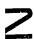
\includegraphics[keepaspectratio]{images/part001_ead1ec0a.jpg}}

即使 \(s \neq \{0\}\)，g 上也可能存在非退化对称双线性形式（习题 18 (c)）。当然，这样的形式并不与 g 的任何表示相关。

推论。设 \(\mathfrak{g},\mathfrak{g}'\) 是李代数，\(\mathfrak{s}\)（分别为 \(\mathfrak{s}'\)）是 \(\mathfrak{g}\)（分别为 \(\mathfrak{g}'\)）的幂零根，\(f\) 是从 \(\mathfrak{g}\) 到 \(\mathfrak{g}'\) 上的一个同态。

\begin{enumerate}
\def\labelenumi{(\alph{enumi})}
\item
  则 \(\mathfrak{s}' = f(\mathfrak{s})\)。
\item
  \(\mathfrak{g}'\) 是约化的，当且仅当 \(f\) 的核包含 \(\mathfrak{s}\)。
\end{enumerate}

若 \(\mathfrak{r},\mathfrak{r}'\) 是 \(\mathfrak{g},\mathfrak{g}',\) 的根基，则 \(\mathfrak{s}' = [\mathfrak{g}',\mathfrak{r}'] = [f(\mathfrak{g}),f(\mathfrak{r})] = f([ \mathfrak{g},\mathfrak{r}]) = f(\mathfrak{s})\)。断言 (b) 是 (a) 的直接推论。

\subsection{应用：表示半单性的判据}

定理 4. 设 \(\mathfrak{g}\) 是李代数，\(\mathfrak{r}\) 是其根基，\(\rho\) 是 \(\mathfrak{g},\mathfrak{g}' = \rho (\mathfrak{g})\) 的有限维表示，且 \(\mathfrak{r}' = \rho (\mathfrak{r})\)。则以下条件等价：

\begin{enumerate}
\def\labelenumi{(\alph{enumi})}
\item
  \(\rho\) 是半单的；
\item
  \(\mathfrak{g}'\) 是约化的，且其中心由半单自同态组成；
\item
  \(\mathfrak{r}'\) 由半单自同态组成；
\item
  \(\rho\) 在 \(\mathfrak{r}\) 上的限制是半单的。
\item
  \(\Rightarrow\) (b)：若 \(\rho\) 是半单的，则 \(\mathfrak{g}'\) 是约化的（命题 5）；由 1 和 \(\mathfrak{g}'\) 生成的结合代数是半单的（《代数》VIII 章，§ 5，第 1 号，命题 3），所以其中心是半单的（同上引文，§ 5，第 4 号，命题 12），从而该中心的元素都是半单的（同上引文，§ 9，第 1 号，命题 2）。
\item
  \(\Rightarrow\) (c)：若 \(\mathfrak{g}'\) 是约化的，则其中心等于其根基，即 \(\mathfrak{r}'\)，于是得到蕴含 (b) \(\Rightarrow\) (c)。
\item
  \(\Rightarrow\) (d)：假设 \(\mathfrak{r}'\) 由半单自同态组成。由于 \([\mathfrak{g}',\mathfrak{r}']\) 由幂零自同态组成（第 4 号，命题 6），有 \([\mathfrak{g}',\mathfrak{r}'] = \{0\}\)。然后，蕴含 (c) \(\Rightarrow\) (d) 由《代数》VIII 章§ 9，第 2 号，定理 1 得到。
\item
  \textgreater{} (a)：令 \(\mathfrak{s}\) 为 \(\mathfrak{g}\) 的幂零根，\(\rho'\) 为 \(\rho\) 在 \(\mathfrak{r}\) 上的限制。由于 \(\rho(\mathfrak{s})\) 的元素都是幂零的，\(\mathfrak{s}\) 包含于 \(\rho'\) 的最大幂零理想中。由于 \(\rho'\) 是半单的，\(\rho'(\mathfrak{s}) = \{0\}\)，而 \(\mathfrak{g}'\) 是约化的（命题 6 的推论），所以 \(\mathfrak{g}' = \mathfrak{a}' \times \mathfrak{r}'\)，其中 \(a'\) 是半单的（命题 5）。令 \(\mathbf{A}'\)（分别为 \(\mathbf{R}'\)）为由 1 和 \(a'\)（分别为 \(\mathfrak{r}'\)）生成的结合代数。它是半单的（《代数》VIII 章，§ 5，第 1 号，命题 3），因而 \(\mathbf{A}' \otimes_{\mathbb{K}} \mathbf{R}'\) 是半单的（同上引文，§ 7，第 6 号，定理 3 的推论 4），从而由 1 和 \(\mathfrak{g}'\) 生成的结合代数（它是 \(\mathbf{A}' \otimes_{\mathbb{K}} \mathbf{R}'\) 的一个商）是半单的，这就证明了 \(\rho\) 是半单的。
\end{enumerate}

推论 1. 设 g 是李代数，\(\rho\) 和 \(\rho'\) 是 g 的两个有限维半单表示。则 \(\rho\) 与 \(\rho'\) 的张量积是半单的。

令 \(\mathfrak{r}\) 为 \(\mathfrak{g}\) 的根基。对于 \(x \in \mathfrak{r}\)，\(\rho(x)\) 和 \(\rho'(x)\) 都是半单的（定理 4），因而 \(\rho(x) \otimes 1 + 1 \otimes \rho'(x)\) 是半单的（《代数》VIII 章§ 9，定理 1 的推论），所以 \(\rho\) 与 \(\rho'\) 的张量积是半单的（定理 4）。

推论 2. 设 \(\mathfrak{g}\) 是李代数，\(\rho\) 是 \(\mathfrak{g}\) 在有限维向量空间 \(V\) 上的半单表示，\(T\) 和 \(S\) 是 \(V\) 的张量代数与对称代数，\(\sigma_{T}\) 和 \(\sigma_{S}\) 是 \(\mathfrak{g}\) 在 \(T\) 和 \(S\) 上由 \(\rho\) 规范导出的表示。则 \(\sigma_{T}\) 和 \(\sigma_{S}\) 是半单的；更确切地说，它们是有限维单表示的直和。

令 \(T^{n}\) 为 T 中由 n 阶齐次张量组成的子空间。~该子空间在 \(\sigma_{T}\) 下稳定，而 \(\sigma_{T}\) 在 \(T^{n}\) 上定义的表示是半单的（推论 1）。因此关于 \(\sigma_{T}\) 的推论成立，从而关于 \(\sigma_{S}\) 的推论也成立，因为后者是 \(\sigma_{T}\) 的一个商表示。

推论 3. 设 g 是李代数，\(\rho\) 和 \(\rho'\) 是 g 在 M 和 M' 上的两个有限维半单表示。g 在 \(\mathcal{L}_{\mathrm{k}}(\mathrm{M},\mathrm{M}')\) 上的表示是由 \(\rho\) 和 \(\rho'\) 规范导出的，因而是半单的。

g-模 \(\mathcal{L}_{\mathbb{K}}(\mathbf{M},\mathbf{M}^{\prime})\) 可规范地与 g-模 \(\mathbf{M}^{*}\otimes_{\mathbb{K}}\mathbf{M}^{\prime}\) 等同（§ 3，第 3 号，命题 4），所以推论 3 由推论 1 得到。

推论 4. 设 \(\mathfrak{g}\) 是李代数，a 是 \(\mathfrak{g}\) 的一个理想，\(\rho\) 是 \(\mathfrak{g}\) 的半单表示。

\begin{enumerate}
\def\labelenumi{(\alph{enumi})}
\item
  \(\rho'\) 为 \(\rho\) 在 a 上的限制是半单的。
\item
  若 \(\rho\) 是单的，则 \(\rho'\) 是彼此同构的单表示之和。
\end{enumerate}

将 \(\rho\) 对其核取商后，可以假设 \(\rho\) 是忠实的。于是 \(\mathfrak{g}\) 是约化的。令 \(\mathfrak{g} = \mathfrak{g}_1 \times \mathfrak{g}_2\)，其中 \(\mathfrak{g}_1\) 是 \(\mathfrak{g}\) 的中心，\(\mathfrak{g}_2\) 是半单的。于是 \(\mathfrak{a} = \mathfrak{a}_1 \times \mathfrak{a}_2\)，其中 \(\mathfrak{a}_1 \subset \mathfrak{g}_1\)，\(\mathfrak{a}_2 \subset \mathfrak{g}_2\)，且 \(\mathfrak{a}_1\) 是 \(\mathfrak{a}\) 的中心。\(\rho(\mathfrak{g}_1)\) 的元素，特别是 \(\rho(\mathfrak{a}_1)\) 的元素，都是半单的（定理 4），因而 \(\rho\) 是半单的（定理 4）。于是得到 (a)。断言 (b) 由 (a) 得到，应用§3，第 1 号，命题 1 的推论。

\subsection{在李代数中约化的子代数}

定义 5. 设 g 是李代数，h 是 g 的李子代数。如果表示 \(x \mapsto ad_{g} x\) 给出的 h 在 g 上的表示是半单的，则称 h 在 g 中是约化的。

该表示包含 \(\mathfrak{h}\) 的伴随表示作为子表示。因此，若 \(\mathfrak{h}\) 在 \(\mathfrak{g},\mathfrak{h}\) 中是约化的，则它是约化的。另一方面，说一个李代数在自身中约化，等价于说它是约化的。

命题 7. 设 g 是李代数，h 是在 g 中约化的子代数，ρ 是 g 在向量空间 V 上的一个表示，W 是 V 中所有作为有限维单 h-模的子空间之和。则 W 在 ρ(g) 下稳定。

令 \(W_0\) 为 V 的有限维单 \(\mathfrak{h}\)-子模。我们要证明关系 \(\rho(x)(W_0) \subset W\) 对所有 \(x \in \mathfrak{g}\) 成立。令 M 表示向量空间 \(\mathfrak{g}\)，将其视为 \(\mathfrak{h}\)-模，所依据的是 \(x \mapsto \operatorname{ad}_{\mathfrak{g}} x\) 给出的 \(\mathfrak{h}\) 在 \(\mathfrak{g}\) 上的表示。于是 \(M \otimes_{K} W_0\) 是半单 \(\mathfrak{h}\)-模（定理 4 的推论 1）。令 \(\theta\) 为从 \(\mathbf{M} \otimes_{\mathbb{K}} \mathbf{W}_0\) 到 \(\mathbf{V}\) 的 K-线性映射，由 \(\theta(x \otimes w) = \rho(x)w\) 定义。它是 \(\mathfrak{h}\)-模同态，因为若 \(y \in \mathfrak{h}\) 则：

\[
\begin{array}{r l} \theta ([ y, x ] \otimes w + x \otimes \rho (y) w) & = \rho ([ y, x ]) w + \rho (x) \rho (y) w \\ & = \rho (y) \rho (x) w = \rho (y) \theta (x \otimes w). \end{array}
\]

因此 \(\theta (\mathbf{M}\otimes_{\mathbb{K}}\mathbf{W}_0)\) 是有限维半单 \(\mathfrak{h}\)-模。因此 \(\theta (\mathbf{M}\otimes_{\mathbb{K}}\mathbf{W}_0)\subset \mathbf{W}\) 包含于 \(\rho (x)(\mathbf{W}_0)\subset \mathbf{W}\)，也就是说对所有 \(x\in \mathfrak{g}\) 都有相应的包含关系。

推论 1. 设 g 是李代数，h 是在 g 中约化的子代数，\(\rho\) 是 g 的有限维半单表示。则 \(\rho\) 在 h 上的限制是半单的。

只需考虑 \(\rho\) 是单的情形。采用命题 4 的记号 V、W。令 \(W_{1}\) 为 V 中在 \(\rho(\mathfrak{h})\) 下稳定的非零子空间中极小的一个。则 \(W_{1} \subset W\)，从而 \(W \neq \{0\}\)，进而 \(W = V\)。

推论 2. 设 g 是李代数，h 是在 g 中约化的子代数，k 是 h 中在 h 内约化的子代数。则 k 在 g 中约化。

表示 \(x \mapsto \operatorname{ad}_{\mathfrak{g}} x\) 给出的 \(\mathfrak{h}\) 在 \(\mathfrak{g}\) 上的表示是半单的，因此它在 \(k\) 上的限制是半单的（推论 1）。

\subsection{半单李代数的例子}

命题 8. 设 V 是有限维向量空间。则 \(\mathfrak{gl}(V)\) 是约化的；其中心是 V 的数乘变换所成的集合，其导出代数是 \(\mathfrak{sl}(V)\)，后者是半单的。

\(\mathfrak{gl}(\mathsf{V})\) 的恒等表示是单的，所以 \(\mathfrak{gl}(\mathsf{V})\) 是约化的，从而 \(\mathfrak{gl}(\mathsf{V})\) 是其中心 \(c\) 与其导出代数 \(\mathcal{D}(\mathfrak{gl}(\mathsf{V}))\) 的直和。中心 \(c\) 是数乘变换的集合（《代数》II 章§2，第 5 号，命题 5 的推论 1）。显然 \(\mathcal{D}(\mathfrak{gl}(\mathsf{V})) \subset \mathfrak{sl}(\mathsf{V})\)。由于 \(\mathfrak{sl}(\mathsf{V}) \cap c = \{0\}\)，\(\mathcal{D}(\mathfrak{gl}(\mathsf{V})) = \mathfrak{sl}(\mathsf{V})\)。因此 \(\mathfrak{sl}(\mathsf{V})\) 是半单的。

例。我们把 \(\mathfrak{sl}(\mathbf{K}^{2})\) 与二阶迹为零矩阵的李代数等同。记

\[
X = \left( \begin{array}{c c} 0 & 1 \\ 0 & 0 \end{array} \right) \qquad Y = \left( \begin{array}{c c} 0 & 0 \\ 1 & 0 \end{array} \right) \qquad H = \left( \begin{array}{c c} 1 & 0 \\ 0 & - 1 \end{array} \right).
\]

于是 \(X, Y, H\) 构成 \(\mathfrak{sl}(\mathbf{K}^2)\) 的一个基，并且

\[
[ H, X ] = 2 X \quad [ H, Y ] = - 2 Y \quad [ X, Y ] = H.
\]

由于维数为 1 或 2 的代数不是半单的（第 1 号，备注 1），\(\mathfrak{sl}(\mathbf{K}^2)\) 是单的。事实上，\(\mathfrak{sl}(\mathbf{V})\) 在 \(\dim V \geqslant 2\) 时是单的，我们稍后将看到这一点（另见习题 21 和 24）。

命题 9. 设 \(\mathrm{V}\) 为维数 \(n\) 的、定义在 \(\mathbf{K}\) 上的有限维向量空间，\(\beta\) 是 \(\mathrm{V}\) 上的非退化对称（分别为交错）双线性形式。令 \(\mathfrak{g}\) 为由 \(x \in \mathfrak{gl}(\mathrm{V})\) 组成的李代数，满足 \(\beta (xm, m') + \beta (m, xm') = 0\) 对所有 \(m, m'\)（属于 \(\mathrm{V}\)）成立。则 \(\mathfrak{g}\) 是约化的；\(\mathfrak{g}\) 是半单的，除非 \(\beta\) 对称且 \(n = 2\)。

对所有 \(u \in \mathfrak{gl}(\mathrm{V})\)，令 \(u^*\) 表示关于 \(\beta\) 的伴随；由《代数》IX 章§ 1，第 8 号的命题 7，有 \(\operatorname{Tr}(u) = \operatorname{Tr}(u^*)\)。条件

\[
\beta (u m, m ^ {\prime}) + \beta (m, u m ^ {\prime}) = 0
\]

对 V 中所有 \(m\)、\(m'\)，\(u + u^{*} = 0\) 成立。特别地，若 \(v \in \mathfrak{gl}(V)\)，则 \((v - v^{*})^{*} = v^{*} - v\)，因而 \(v - v^{*} \in \mathfrak{g}\)。现在令 \(u\) 为 \(\mathfrak{g}\) 中与 \(\mathfrak{g}\) 正交的元素，其中所用的双线性形式 \(\phi\) 与 \(\mathfrak{g}\) 的恒等表示相关。对所有 \(v \in \mathfrak{gl}(V)\)，\(\operatorname{Tr} u(v - v^{*}) = 0\) = 0，所以

\[
\operatorname{Tr} (u v) = \operatorname{Tr} (u v ^ {*}) = \operatorname{Tr} (u v ^ {*}) ^ {*} = \operatorname{Tr} (v u ^ {*}) = - \operatorname{Tr} (v u) = - \operatorname{Tr} (u v)
\]

从而 \(\operatorname{Tr}(u v) = 0\)。这说明 \(u = 0\)，所以 \(\phi\) 非退化。因此 \(\mathfrak{g}\) 是约化的（命题 5）。还需证明 \(\mathfrak{g}\) 的中心为零（除 \(\beta\) 对称且 \(n = 2\) 的情形外）。扩张基域后，可以假设 \(\mathbf{K}\) 是代数闭的。

\begin{enumerate}
\def\labelenumi{(\alph{enumi})}
\item
  当 \(\beta\) 对称时，它可以与 \(\mathbf{K}^n\) 上相对于典范基、矩阵为 \(I_{\mathrm{n}}\) 的双线性形式等同（《代数》IX 章§6，定理 1 的推论 1）。在这些条件下 \(\mathfrak{g}\) 可与斜对称矩阵的李代数等同（§3，第 4 号，例 1）。令 \(U = (u_{ij}) \in \mathfrak{g}\)；我们利用以下事实：\(U\) 与矩阵 \((v_{ij}) \in \mathfrak{g}\) 可交换，该矩阵除 \(v_{i_0j_0}\) 和 \(v_{j_0i_0}\) 外所有元素均为零（\(i_0 \neq j_0\)），且这两个元素分别等于 1 和 -1。我们得到 \(u_{i_0j} = u_{j_0j} = u_{ii_0} = u_{ij_0} = 0\)，当 \(i \neq i_0, j_0\) 且 \(j \neq i_0, j_0\) 时。若 \(n > 2\)，则对所有不同的指标 \(i_0\) 和 \(j\)，存在不同的指标 \(i\) 和 \(j_0\)，使得 \(i \neq i_0, j_0 \neq j, j_0 \neq i_0\)；所以 \(u_{i_0j} = 0\)。这证明 \(\mathfrak{g}\) 的中心元素为零。
\item
  当 \(\beta\) 交错且 \(n = 2m\) 时，\(\beta\) 可以与 \(\mathbf{K}^{2m}\) 上矩阵为 \(\left( \begin{array}{cc}0 & I_m \\ -I_m & 0 \end{array} \right)\) 的双线性形式等同（《代数》IX 章§5，定理 1 的推论 1）。在这些条件下 \(\mathfrak{g}\) 可与形如 \(U = \left( \begin{array}{cc}A & B\\ C & D \end{array} \right)\) 的矩阵李代数等同，其中 \(D = -^t A\)，\(B\) 和 \(C\) 是对称的（\(A, B, C, D\) 属于 \(\mathbf{M}_m(\mathbf{K})\)）（§3，第 4 号，例 1）。首先利用 \(U\) 与矩阵 \(\left( \begin{array}{cc}X & 0 \\ 0 & -^t X \end{array} \right)\) 可交换这一事实，其中 \(X \in \mathbf{M}_m(\mathbf{K})\)。于是 \(AX = X A\)、\(CX = -^t XC\)、\(XB = -B\)。\(^t X\)；由于这些等式必须对所有 \(X\) 成立，因而 \(A\) 是标量矩阵 \(\lambda I_m\)。现在利用 \(U\) 与矩阵 \(\left( \begin{array}{cc}0 & Y \\ 0 & 0 \end{array} \right)\) 可交换这一事实，其中
\end{enumerate}

\(Y\) 是 \(\mathbf{M}_m(\mathrm{K})\) 的对称矩阵。于是 \(\lambda Y = YC = CY = 0\)。这首先证明 \(\lambda = 0\)。此外，对所有 \(X \in \mathbf{M}_m(\mathrm{K})\)，\(X + {}^t X\) 是对称的，因而 \(XC = -{}^t XC\)。利用上面得到的等式 \(CX = -{}^t XC\)，可见 \(C\) 与 \(\mathbf{M}_m(\mathrm{K})\) 的每个元素可交换，所以 \(C\) 是标量矩阵；由于 \(YC = 0\)，它必为零。类似地可证明 \(B = 0\)。

当 \(\beta\) 对称且 \(n = 2\) 时，\(\mathfrak{g}\) 是一维的，因而是交换的。其他情形见习题 25 和 26。

\subsection{Levi--Malcev 定理}

设 E 是 R 上的完备赋范向量空间，u 是 E 的连续自同态。我们已经看到（《实变函数》，第四章，§ 2，第 6 号），序列 \(\frac{u^{n}}{n!}\) 在 \(\mathcal{L}(E)\) 中可求和，并记为

\[
e ^ {u} = \exp u = \sum_ {n = 0} ^ {\infty} \frac {u ^ {n}}{n !}.
\]

现在设 E 是域 K 上的向量空间，u 是 E 的幂零自同态。级数 \(\sum_{n=0}^{\infty}\frac{u^{n}}{n!}\) 只有有限个非零项，因此可写为

\[
e ^ {u} = \exp u = \sum_ {n = 0} ^ {\infty} \frac {u ^ {n}}{n !}.
\]

若 K = R 且 E 是完备赋范的，这一定义与上述定义一致。若 v 是 E 的另一个幂零自同态，且与 u 可交换，则：

\[
\begin{array}{l} e ^ {u} e ^ {v} = \left(\sum_ {n = 0} ^ {\infty} \frac {u ^ {n}}{n !}\right) \left(\sum_ {p = 0} ^ {\infty} \frac {v ^ {p}}{p !}\right) = \sum_ {n, p = 0} ^ {\infty} \frac {u ^ {n} v ^ {p}}{n ! p !} \\ = \sum_ {q = 0} ^ {\infty} \frac {1}{q !} \left(\sum_ {n + p = q} \binom {q} {n} u ^ {n} v ^ {p}\right) = \sum_ {q = 0} ^ {\infty} \frac {1}{q !} (u + v) ^ {q} = e ^ {u + v}. \end{array}\tag{3}
\]

特别地，\(e^u e^{-u} = e^{-u}e^u = e^0 = 1\)，因此 \(e^u\) 总是 E 的自同构。

此外，若 E 是一个（不必结合的）代数，而 u 是 E 的（幂零）导子，则 \(e^{u}\) 是代数 E 的自同构。因为若 \(x, y \in E\)，则

\[
u ^ {p} (x y) = \sum_ {r + s = p} \binom {p} {r} u ^ {r} (x) u ^ {s} (y)
\]

对每个整数 \(p \geqslant 0\) 都成立（Leibniz 公式）。由此

\[
\begin{array}{r l} e ^ {u} (x y) & = \sum_ {p \geqslant 0} \frac {1}{p !} u ^ {p} (x y) = \sum_ {p \geqslant 0} \sum_ {r + s = p} \frac {u ^ {r} (x)}{r !} \frac {u ^ {s} (y)}{s !} \\ & = \sum_ {r, s = 0} ^ {\infty} \frac {u ^ {r} (x)}{r !} \frac {u ^ {s} (y)}{s !} = e ^ {u} (x) e ^ {u} (y) \end{array}
\]

从而得到所述断言。

现在设 g 是李代数。若 x 属于 g 的幂零根，则 g 的导子 \(ad_{g}x\) 是幂零的。因此可作如下定义：

定义 6. g 的特殊自同构是形如 \(e^{ad_{\mathfrak{g}} x}\) 的 g 的自同构，其中 x 属于 g 的幂零根。

显然，特殊自同构使 g 的每个理想保持稳定。

定义 7. 设 \(\mathfrak{g}\) 是李代数，\(\mathfrak{r}\) 是其根基。\(\mathfrak{g}\) 的 Levi 子代数是 \(\mathfrak{g}\) 中任意一个以 \(\mathfrak{r}\) 为补的子代数。

Levi 子代数同构于 \(\mathfrak{g} / \mathfrak{r}\)，因而是半单的。半单子代数与 \(\mathfrak{r}\) 的交只有 0；因此，任意半单子代数 \(\mathfrak{h}\)，只要满足 \(\mathfrak{g} = \mathfrak{r} + \mathfrak{h}\)，就是 Levi 子代数；所以，Levi 子代数在满同态下的像仍是 Levi 子代数。

定理 5 (Levi--Malcev). 李代数 g 总有一个 Levi 子代数 s。g 的每个 Levi 子代数都是 s 在某个特殊自同构下的像。

令 r 表示 g 的根基。我们先处理两种特殊情形。

\begin{enumerate}
\def\labelenumi{(\alph{enumi})}
\tightlist
\item
  \([g, r] = \{0\}\) .
\end{enumerate}

根据命题 5，此时 g 是其中心 r 与半单的 Dg 的乘积。因此 Dg 是 Levi 子代数。此外，若 \(s'\) 是半单子代数，则 \(s' = Ds'\)（定理 1），从而 \(s' \subset Dg\)；因此 Dg 是 g 的唯一 Levi 子代数。

\begin{enumerate}
\def\labelenumi{(\alph{enumi})}
\setcounter{enumi}{1}
\tightlist
\item
  \([\mathfrak{g},\mathfrak{r}]\neq \{0\}\)，且 \(\mathfrak{g}\) 中包含于 \(\mathfrak{r}\) 的理想只有 \(\{0\}\) 和 \(\mathfrak{r}\)。
\end{enumerate}

于是 \([\mathfrak{g},\mathfrak{r}] = \mathfrak{r}\)，\([\mathfrak{r},\mathfrak{r}] = \{0\}\)，且 \(\mathfrak{g}\) 的中心为零。令 M（分别为 N）为 \(\mathcal{L}(\mathfrak{g})\) 的子空间，由 \(\mathfrak{g}\) 映入 \(\mathfrak{r}\) 的线性映射组成；这些映射在 \(\mathfrak{r}\) 上的限制分别为数乘变换（分别为零），故 N 在 M 中余维为 1。对于 \(m\in M\)，令 \(\lambda (m)\) 表示 \(\mathfrak{r}\) 上由 \(m\) 定义的数乘变换的比值。令 \(\sigma\) 为 \(\mathfrak{g}\) 在 \(\mathcal{L}(\mathfrak{g})\) 上由伴随表示规范导出的表示；回忆有 \(\sigma (x).u = [\mathrm{ad}_{\mathfrak{g}}x,u]\)，其中 \(x\in \mathfrak{g}\) 且 \(u\in \mathcal{L}(\mathfrak{g})\)。

\[
\mathcal{L}(\mathfrak{g}) \supset \mathrm{M} \supset \mathrm{N} \supset \mathrm{P}
\]
显然，\(\sigma (x)(\mathrm{M})\subset \mathrm{N}\) 对所有 \(x\in \mathfrak{g}\) 都成立。此外，若 \(x\in \mathfrak{r},y\in \mathfrak{g}\) 且 \(u\in \mathrm{M}\)，则\\
（4）\((\sigma (x).u)(y) = [x,u(y)] - u([x,y]) = -\lambda (u)[x,y]\)，因为 \([\mathfrak{r},\mathfrak{r}] = \{0\}\)；式（4）可写为：\\
（5）\(\sigma (x).u = -\mathrm{ad}(\lambda (u).x)\)。

由于 g 的中心为零，映射 \(x \mapsto ad_{g}x\) 定义了一个双射 \(\phi\)，把 r 映到 \(\mathcal{L}(\mathfrak{g})\) 的一个子空间 P 上。这个子空间在 \(\sigma(\mathfrak{g})\) 下稳定，并包含于 N 中，因为 r 是交换理想；由（5）可知，\(\sigma(x)(\mathrm{M}) \subset \mathrm{P}\) 对 \(x \in \mathfrak{r}\) 成立。由 \(\sigma\) 在 M/P = V 上导出的表示因此在 r 上为零，并定义了半单代数 g/r 在 V 上的表示 \(\sigma'\)。对于所有 \(y \in g/r\)，空间 \(\sigma'(y)(V)\) 包含于 N/P 中，后者在 V 中余维为 1。因此（第 2 号，引理 3），存在 \(u_{0} \in M\)，使 \(\lambda(u_{0}) = -1\)，且 \(\sigma(x).u_{0} \in P\) 对所有 \(x \in g\) 都有。映射 \(x \mapsto \phi^{-1}(\sigma(x).u_{0})\) 是从 \(x \in g\) 到 r 的线性映射。根据（5），它在 r 上的限制是 r 的恒等映射。因此它的核是 g 中以 r 为补的子空间 s。由于 s 正是满足 \(\sigma(x).u_{0} = 0\) 的 x 的集合，所以 s 是 g 的子代数，因而是 g 的 Levi 子代数。

令 \(\mathfrak{s}'\) 是另一个 Levi 子代数。对每个 \(x \in \mathfrak{s}'\)，令 \(h(x)\) 为 \(\mathfrak{r}\) 中满足 \(x + h(x) \in \mathfrak{s}\) 的唯一元素。由于 \(\mathfrak{s}\) 是子代数且 \(\mathfrak{r}\) 交换，对于 \(x, y\)（属于 \(\mathfrak{s}'\)），有：

\[
[ x + h (x), y + h (y) ] = [ x, y ] + [ x, h (y) ] + [ h (x), y ] \in \mathfrak {s}
\]

因此

\[
h ([ x, y ]) = (\operatorname{ad} x). h (y) - (\operatorname{ad} y). h (x).
\]

根据第 2 号的备注 2，存在 \(a \in \mathfrak{r}\)，使 \(h(x) = -[x, a]\) 对所有 \(x \in \mathfrak{s}'\) 成立。于是：

\[
x + h (x) = x + [ a, x ] = (1 + \operatorname{ad} a). x.\tag{6}
\]

由于 \(\mathfrak{r}\) 交换，\((\operatorname{ad} a)^2 = 0\)，所以 \(1 + \operatorname{ad} a = e^{\operatorname{ad} a}\)。由于 \(\mathfrak{r} = [\mathfrak{s}, \mathfrak{r}]\)，\(e^{\operatorname{ad} a}\) 是 \(\mathfrak{g}\) 的特殊自同构。根据（6），此特殊自同构把 \(\mathfrak{s}'\) 映到 \(\mathfrak{s}\)。

\textbf{(c) 一般情形：}

我们对根基的维数 \(n\) 作归纳。当 \(n = 0\) 时无事可证，因此可假设定理对根基维数小于 \(<\dim \mathfrak{r}\) 的李代数成立。由（a），只需考虑 \([\mathfrak{g}, \mathfrak{r}] \neq \{0\}\) 的情形。由于 \([\mathfrak{g}, \mathfrak{r}]\) 是幂零的（第 4 号，命题 6），其中心 \(\mathfrak{c}\) 是非零的，即满足 \(\neq \{0\}\)。令 \(\mathfrak{m}\) 为 \(\mathfrak{g}\) 中包含于 \(\mathfrak{c}\) 的极小非零理想。若 \(\mathfrak{m} = \mathfrak{r}\)，则为情形（b）。因此设 \(\mathfrak{m} \neq \mathfrak{r}\)，并令 \(f\) 为从 \(\mathfrak{g}\) 映到 \(\mathfrak{g}' = \mathfrak{g}/\mathfrak{m}\) 的典范映射。\(\mathfrak{g}'\) 的根基是 \(\mathfrak{r}' = \mathfrak{r}/\mathfrak{m}\)。由归纳假设，\(\mathfrak{g}'\) 有 Levi 子代数 \(\mathfrak{h}'\)。于是 \(\mathfrak{h} = f^{-1}(\mathfrak{h}')\) 是 \(\mathfrak{g}\) 的子代数，包含 \(\mathfrak{m}\)，且 \(\mathfrak{h}/\mathfrak{m} = \mathfrak{h}'\) 是半单的，因而其根基为 \(\mathfrak{m}\)。由归纳假设，\(\mathfrak{h} = \mathfrak{m} + \mathfrak{s}\)，其中 \(\mathfrak{s}\) 是半单子代数。等式 \(\mathfrak{g}' = \mathfrak{r}' + \mathfrak{h}'\) 蕴含 \(\mathfrak{g} = \mathfrak{r} + \mathfrak{h} = \mathfrak{r} + \mathfrak{m} + \mathfrak{s} = \mathfrak{r} + \mathfrak{s}\)，从而 \(\mathfrak{s}\) 是 \(\mathfrak{g}\) 的 Levi 子代数。

令 \(\mathfrak{s}'\) 是 \(\mathfrak{g}\) 的另一个 Levi 子代数。则 \(f(\mathfrak{s})\) 和 \(f(\mathfrak{s}')\) 是 \(\mathfrak{g}'\) 的两个 Levi 子代数；由归纳假设，存在 \(a' \in [\mathfrak{g}', \mathfrak{r}']\)，使 \(e^{\mathrm{ad} a'}(f(\mathfrak{s}')) = f(\mathfrak{s})\)。若存在 \(a \in [\mathfrak{g}, \mathfrak{r}]\) 使 \(f(a) = a'\)，则可得：

\[
\mathfrak {s} _ {1} = e ^ {\mathrm{ad} a} \left(\mathfrak {s} ^ {\prime}\right) \subset \mathfrak {m} + \mathfrak {s} = \mathfrak {h}.
\]

于是 \(\mathfrak{s}_1\) 和 \(\mathfrak{s}\) 是 \(\mathfrak{h}\) 的两个 Levi 子代数。由归纳假设，存在 \(b\in \mathfrak{m}\)，使 \(e^{\mathrm{ad}b}(\mathfrak{s}_1) = \mathfrak{s}\)。因此 \(\mathfrak{s} = e^{\mathrm{ad}b}.e^{\mathrm{ad}a}(\mathfrak{s}')\)。最后，由于 \(\mathfrak{m}\) 位于 \([\mathfrak{g},\mathfrak{r}]\) 的中心，\(e^{\mathrm{ad}b}.e^{\mathrm{ad}a} = e^{\mathrm{ad}(b + a)}\)，且 \(b + a\in [\mathfrak{g},\mathfrak{r}]\)，这就完成了证明。

推论 1. 设 \(\mathfrak{s}\) 是 \(\mathfrak{g}\) 的 Levi 子代数，\(\mathfrak{h}\) 是 \(\mathfrak{g}\) 的半单子代数。

\begin{enumerate}
\def\labelenumi{(\alph{enumi})}
\item
  存在 \(\mathfrak{g}\) 的一个特殊自同构，把 \(\mathfrak{h}\) 映到 \(\mathfrak{s}\) 的一个子代数上。
\item
  \(\mathfrak{h}\) 包含于 \(\mathfrak{g}\) 的某个 Levi 子代数中。
\end{enumerate}

令 \(\mathfrak{r}\) 为 \(\mathfrak{g}\) 的根基，令 \(\mathfrak{a} = \mathfrak{h} + \mathfrak{r}\)；它是 \(\mathfrak{g}\) 的子代数。于是 \(\mathfrak{a}/\mathfrak{r}\) 是半单的，而 \(\mathfrak{r}\) 可解，所以 \(\mathfrak{r}\) 是 \(\mathfrak{a}\) 的根基，且 \(\mathfrak{h}\) 是 \(\mathfrak{a}\) 的 Levi 子代数。另一方面，\(\mathfrak{a} \cap \mathfrak{s} = \mathfrak{h}'\) 以 \(\mathfrak{r}\) 为补，是 \(\mathfrak{a}\) 中的一个子代数，因而也是 \(\mathfrak{a}\) 的 Levi 子代数。于是（定理 5）存在 \(a \in [\mathfrak{a}, \mathfrak{r}]\)，使 \(e^{\mathrm{ad} a}\) 把 \(\mathfrak{h}\) 映到 \(\mathfrak{h}'\)。现在 \(a \in [\mathfrak{g}, \mathfrak{r}]\)；\(e^{\mathrm{ad} a}\) 把 \(\mathfrak{h}\) 映到 \(\mathfrak{s}\) 的一个子代数中，而 \(e^{-\mathrm{ad} a}(\mathfrak{s})\) 是 \(\mathfrak{g}\) 的 Levi 子代数，包含 \(\mathfrak{h}\)。

推论 2. 对于子代数 \(\mathfrak{h}\)，要成为 \(\mathfrak{g}\) 的 Levi 子代数，充要条件是它成为 \(\mathfrak{g}\) 的极大半单子代数；换言之，\(\mathfrak{h}\) 是 \(\mathfrak{g}\) 中的极大半单子代数。

这直接由推论 1 得到。

推论 3. 设 g 是李代数，m 是 g 的理想，且 g/m 是半单的。则 g 含有一个在 g 中以 m 为补的子代数。换句话说，半单李代数的每个扩张都是非本质的。

令 \(\mathfrak{s}\) 为 \(\mathfrak{g}\) 的 Levi 子代数（定理 5）。它在 \(\mathfrak{g}/\mathfrak{m}\) 中的典范像是一个 Levi 子代数，因而等于 \(\mathfrak{g}/\mathfrak{m}\)，从而 \(\mathfrak{g} = \mathfrak{s} + \mathfrak{m}\)。于是，\(\mathfrak{s}\) 中的一个理想，在 \(\mathfrak{s}\) 中以 \(\mathfrak{m} \cap \mathfrak{s}\) 为补，是 \(\mathfrak{g}\) 中以 \(\mathfrak{m}\) 为补的子代数，且位于 \(\mathfrak{g}\) 中。

推论 4. 设 g 是李代数，r 是其根基，s 是 g 的 Levi 子代数，m 是 g 的理想。则 m 是 m ∩ r（它是 m 的根基）与 m ∩ s（它是 m 的 Levi 子代数）的直和。

我们知道 \(\mathfrak{m} \cap \mathfrak{s}\) 是 \(\mathfrak{m}\) 的根基（§ 5，第 5 号，命题 5 的推论 3）。令 \(\mathfrak{h}\) 为 \(\mathfrak{m}\) 的 Levi 子代数，令 \(\mathfrak{s}'\) 为 \(\mathfrak{g}\) 中包含 \(\mathfrak{h}\) 的 Levi 子代数（推论 1）。代数 \(\mathfrak{m} \cap \mathfrak{s}'\) 是 \(\mathfrak{s}'\) 的理想，因而是半单的；它包含 \(\mathfrak{h}\)，所以等于 \(\mathfrak{h}\)。于是 \(\mathfrak{m}\) 是 \(\mathfrak{m} \cap \mathfrak{r}\) 与 \(\mathfrak{m} \cap \mathfrak{s}'\) 的直和。存在特殊自同构把 \(\mathfrak{s}'\) 映到 \(\mathfrak{s}\)；该自同构保持 \(\mathfrak{r}\) 和 \(\mathfrak{m}\) 不变；因此 \(\mathfrak{m}\) 是 \(\mathfrak{m} \cap \mathfrak{r}\) 与 \(\mathfrak{m} \cap \mathfrak{s}\) 的直和，而 \(\mathfrak{m} \cap \mathfrak{s}\) 是 \(\mathfrak{m}\) 的 Levi 子代数。

\subsection{不变量定理}

设 g 是李代数，\(\rho\) 是 g 在向量空间 M 上的一个表示。对于 g 的每个单表示类 \(\delta\)，令 \(M_{\delta}\) 为 M 的 \(\delta\) 型分量。M 的不变元子空间 \(M_{0}\) 正是 \(M_{\delta_{0}}\)，其中 \(\delta_{0}\) 表示 g 在一维空间上的零表示类。

引理 4. 设 \(\rho, \sigma, \tau\) 是 \(\mathfrak{g}\) 在向量空间 \(\mathbf{M}, \mathbf{N}, \mathbf{P}\) 上的表示。假设给定一个 K-双线性映射 \((m, n) \mapsto m \cdot n\)，它把 \(\mathbf{M} \times \mathbf{N}\) 映入 \(\mathbf{P}\)，并满足

\[
(\rho (x) m). n + m. (\sigma (x) n) = \tau (x) (m. n)
\]

对所有 \(m \in M\)、\(n \in N\) 和 \(x \in g\) 都成立。

\begin{enumerate}
\def\labelenumi{(\alph{enumi})}
\item
  若 \(m_0 \in \mathbf{M}_0\)，则映射 \(n \mapsto m_0\).\(n\) 是 \(\mathfrak{g}\)-模同态。
\item
  若 \(n \in N_{\delta}\)，则 \(m_{0}.n \in P_{\delta}\)。
\item
  若 \(\mathbf{M}\) 是一个（不必结合的）代数，且 \(\rho(x)\) 是 \(\mathbf{M}\) 的导子，同时 \(\mathbf{M}_0\) 是 \(\mathbf{M}\) 的子代数，则每个 \(\mathbf{M}_{\delta}\) 都是 \(\mathbf{M}_0\) 的左、右模。
\end{enumerate}

对于 \(m_{0} \in M_{0}, n \in N\) 和 \(x \in g,\)，有：

\[
\tau (x) \left(m _ {0}. n\right) = m _ {0}. (\sigma (x) n),
\]

因此得到（a）。断言（b）由（a）推出（《代数》，第八章，§ 3，第 4 号，命题 10）。若 \(\mathbf{N} = \mathbf{P} = \mathbf{M}\) 且 \(\sigma = \tau = \rho\)，则断言（b）给出断言（c），作为特殊情形。

引理 5. 进一步设 \(\sigma\) 和 \(\tau\) 是半单的，因而 N（分别为 P）是 \(N_{\delta}\)（分别为 \(P_{\delta}\)）的直和。对于所有 \(n \in N\)（分别对于 \(p \in P\)），令 \(n^{\sharp}\)（分别为 \(p^{\sharp}\)）表示它在 \(N_0\)（分别为 \(P_0\)）中的分量。设 \(m_0 \in M_0\)。则对所有 \(n \in N\)，有 \((m_0.n)^{\sharp} = m_0.n^{\sharp}\)。

由线性性，只需考虑 \(n \in \mathrm{N}_{\delta}\) 的情形。若 \(\delta \neq \delta_0\)，则 \(n^{\sharp} = 0\)，且由引理 4，\(m_0.n \in \mathrm{P}_{\delta}\)，所以 \((m_0.n)^{\sharp} = 0 = m_0.n^{\sharp}\)。若 \(\delta = \delta_0\)，则 \(n^{\sharp} = n\)，且由引理 4，\(m_0.n \in \mathrm{P}_0\)，所以 \((m_0.n)^{\sharp} = m_0.n = m_0.n^{\sharp}\)。

定理 6. 设 \(\mathfrak{g}\) 是李代数，V 是 \(\mathfrak{g}\)-模，是 K 上的有限维半单模；S 是 V 的对称代数，\(x_{\mathrm{S}}\) 是 S 上延拓 \(x_{\mathrm{V}}\) 的导子（从而 \(x \mapsto x_{\mathrm{S}}\) 是 \(\mathfrak{g}\) 在 S 上的一个表示）。

\begin{enumerate}
\def\labelenumi{(\alph{enumi})}
\item
  \(\mathbf{S}_0\) 的不变量代数 \(\mathbf{S}\) 由有限个元素生成。
\item
  对于每个单表示类 \(\delta\)（它是 \(\mathfrak{g}\) 的、且在 \(\mathbf{K}\) 上有限维的单表示类），令 \(\mathrm{S}_{\delta}\) 为 \(\mathrm{S}\) 的 \(\delta\) 型分量。则 \(\mathrm{S}_{\delta}\) 是有限生成的 \(\mathrm{S}_{0}\)-模。
\end{enumerate}

令 \(\overline{\mathbf{S}}\subset \mathbf{S}\) 为 S 中无常数项元素构成的理想。令 I 为由 \(\mathrm{S}_0\cap \overline{\mathrm{S}}\) 生成的 S 的理想，令 \((s_1,s_2,\ldots ,s_p)\) 为 I 的一组有限生成元（《交换代数》，第三章，§ 3）。可以假设 \(s_t\) 属于 \(\mathbf{S}_0 \cap \bar{\mathbf{S}}\) 且是齐次的（\(x_{\mathrm{S}}\) 保持次数，因而每个 \(\mathbf{S}_0\) 都是分次子模）。令 \(\mathbf{S}_1\) 为 \(\mathbf{S}\) 的子代数，由 1 和 \(s_t\) 生成。于是 \(\mathbf{S}_1 \subset \mathbf{S}_0\)。我们证明 \(\mathbf{S}_1 = \mathbf{S}_0\)。为此，我们证明：每个齐次元素 \(s\) 若属于 \(\mathbf{S}_0\)，便属于 \(\mathbf{S}_1\)；证明按 \(n\)（即 \(s\) 的次数）归纳。若 \(n = 0\)，断言显然成立。设 \(n > 0\)，并假设当次数小于 n（即 \(< n\)）时断言已成立。由于 \(s \in I\)，有 \(s = \sum_{i=1}^{p} s_i s_i'\)，其中 \(s_i'\) 是 S 中的元素，并可设为齐次的，且 \(\deg(s_i') = \deg(s) - \deg(s_i) < n\)。

\[
s = s ^ {\sharp} = \sum_ {i = 1} ^ {p} (s _ {i} s _ {i} ^ {\prime}) ^ {\sharp} = \sum_ {i = 1} ^ {p} s _ {i} {s _ {i} ^ {\prime}} ^ {\sharp}.
\]

\(s_i^\sharp\) 是 \(S_0\) 中次数 \(< n\) 的齐次元素（因为每个 \(S_\delta\) 都是分次子模），因此根据归纳假设它们属于 \(S_1\)。所以 \(s \in S_1\)，从而证明（a）。

现在考察 g 的一个 \(\delta\) 类的单表示，它作用在有限维空间 M 上。令 \(L = \mathcal{L}_{\mathbb{K}}(M, S)\)。对于所有 \(s \in S\) 和所有 \(f \in L\)，令 sf 为 L 中由 \((sf)(m) = s.f(m)\) 定义的元素（\(m \in M\)）；于是 L 上定义了 S-模结构。由于 M 在 K 上有限维，显然 L 是有限生成的 S-模，因而是诺特 S-模（因为环 S 是诺特的）。另一方面，L 具有规范的 g-模结构。对每个整数 \(n \geqslant 0\)，令 \(S^{n}\) 为 S 中次数 n 的齐次元素集合；于是，g-模 \(\mathcal{L}_{\mathbb{K}}(M, S^{n})\) 是半单的（第 5 号，定理 4 的推论 3），因而 g-模 L 是半单的。此外，对于 \(s \in S\)、\(f \in L\)、\(x \in g\) 和 \(m \in M\)，

\[
\begin{array}{r l} (x _ {\mathrm{L}} (s f)) (m) & = x _ {\mathrm{S}} ((s f) (m)) - (s f) (x _ {\mathrm{M}} m) \\ & = x _ {\mathrm{S}} (s. f (m)) - s. f (x _ {\mathrm{M}} m) \\ & = (x _ {\mathrm{S}} s). f (m) + s. (x _ {\mathrm{S}} f (m)) - s. f (x _ {\mathrm{M}} m) \\ & = ((x _ {\mathrm{S}} s) f) (m) + (s (x _ {\mathrm{L}} f)) (m) \end{array}
\]

从而 \(x_{\mathrm{L}}(sf) = (x_{\mathrm{S}}s)f + s(x_{\mathrm{L}}f)\)。因此可应用引理 5。

L 的不变元子集 \(\mathbf{L}_0\) 正是 \(\mathbf{L}\) 中从 \(g\)-模 \(\mathbf{M}\) 到 \(g\)-模 \(\mathbf{S}\) 的同态集合。因此，若 \(\phi\) 表示从 \(\mathrm{M} \otimes_{\mathrm{K}} \mathrm{L}\) 到 \(\mathrm{S}\) 的规范同态，则 \(\phi(\mathrm{M} \otimes_{\mathrm{K}} \mathrm{L}_0) = \mathrm{S}_{\delta}\)。由于 \(\phi\) 显然是 S-模同态，只需证明 \(\mathbf{L}_0\) 是有限生成的 \(\mathrm{S}_0\)-模。令 \(\mathbf{J}\) 为 \(\mathbf{L}\) 的由 \(\mathbf{L}_0\) 生成的 S-子模。由于 \(\mathbf{L}\) 是诺特 S-模，存在一个有限序列 \((f_1, \ldots, f_q)\)，其元素属于 \(\mathbf{L}_0\)，并生成 S-模 \(\mathbf{J}\)。令 \(\mathbf{L}_1\) 为 \(\mathrm{S}_0\)-模，由 \(f_{1},\ldots ,f_{q}\) 生成。于是 \(\mathrm{L}_1\subset \mathrm{L}_0\)。另一方面，若 \(f\in \mathrm{L}_0\)，则 \(f = \sum_{i = 1}^{q}s_{i},f_{i}\)，其中 \(s_i\in S\) 对所有 \(i\) 成立；因此，根据引理 5（沿用其记号）：

\[
f = f ^ {\sharp} = \left(\sum_ {i = 1} ^ {q} s _ {i} f _ {i}\right) ^ {\sharp} = \sum_ {i = 1} ^ {q} s _ {i} ^ {\sharp} f _ {i} \in L _ {1}.
\]

因此 \(L_{0} = L_{1}\)，所以 \(L_{0}\) 是有限生成的 \(S_{0}\)-模。

\subsection{基域的改变}

设 \(K_{1}\) 是 K 的交换扩域。对于 K 上的李代数 g，它为半单的充要条件是 \(g_{(K_{1})}\) 为半单；因为 \(\beta_{1}\) 是 \(g_{(K_{1})}\) 的 Killing 形式，它由 g 的 Killing 形式 \(\beta\) 将基域从 K 扩张到 \(K_{1}\) 得到；因此，\(\beta_{1}\) 非退化当且仅当 \(\beta\) 非退化（《代数》，第九章，§ 1，第 4 号，命题 3 的推论）。

若 \(\mathfrak{g}_{(\mathbf{K}_{1})}\) 是单的，则根据上文 g 是半单的，且不可能是两个非零理想的乘积，因而 g 是单的。另一方面，即使 g 是单的，\(\mathfrak{g}_{(\mathbf{K}_{1})}\)（它是半单的）也可能不是单的（练习 17 和 26(b)）。

设 \(\mathfrak{g}\) 是李代数，\(\mathfrak{r}\) 是其根基。则 \(\mathfrak{r}_{(\mathbf{K}_1)}\) 是 \(\mathfrak{g}_{(\mathbf{K}_1)}\) 的根基（§ 5，第 6 号）。因此，若 \(\mathfrak{s}\) 表示 \(\mathfrak{g}\) 的幂零根，则 \(\mathfrak{g}_{(\mathbf{K}_1)}\) 的幂零根为 \([\mathfrak{g}_{(\mathbf{K}_1)},\mathfrak{r}_{(\mathbf{K}_1)}] = [\mathfrak{g},\mathfrak{r}]_{(\mathbf{K}_1)} = \mathfrak{s}_{(\mathbf{K}_1)}\)。由此可知，\(\mathfrak{g}\) 是约化的当且仅当 \(\mathfrak{g}_{(\mathbf{K}_1)}\) 是约化的。

设 \(\mathfrak{g}\) 是李代数，\(\mathfrak{h}\) 是其子代数。回忆，\(\mathfrak{h}\) 的一个表示是半单的，当且仅当由 \(\mathfrak{h}_{(\mathrm{K}_1)}\)（基域扩张到 \(\mathrm{K}_1\)）得到的表示是半单的。因此，\(\mathfrak{h}\) 在 \(\mathfrak{g}\) 中约化，当且仅当 \(\mathfrak{h}_{(\mathrm{K}_1)}\) 在 \(\mathfrak{g}_{(\mathrm{K}_1)}\) 中约化。

现在设 \(K_{0}\) 是 K 的子域，且 \([K:K_{0}]\) 有限。令 g 为李代数，\(g_{0}\) 为把基域从 K 限制到 \(K_{0}\) 后由 g 得到的（有限维）李代数。g 的每个交换理想都是 \(g_{0}\) 的交换理想；反之，若 \(a_{0}\) 是 \(g_{0}\) 的交换理想，则 g 中包含 \(a_{0}\) 的最小 K-向量子空间是 g 的交换理想；因此 g 是半单的当且仅当 \(g_{0}\) 是半单的。若 \(g_{0}\) 是单的，显然 g 是单的。反过来，设 g 是单的。我们证明 \(g_{0}\) 是单的。令 \(a_{0}\) 是 \(g_{0}\) 的一个单分量。对所有 \(\lambda \in K^{*}\)，\(\lambda a_{0}\) 是 \(g_{0}\) 的理想，并且

\[
\left[ a _ {0}, \lambda a _ {0} \right] = \lambda \left[ a _ {0}, a _ {0} \right] = \lambda a _ {0} \neq \{0 \},
\]

因而 \(\lambda a_0 \supset a_0\)，并由 \(\lambda a_0 = a_0\)（因为 \(\dim_{K_0}(\lambda a_0) = \dim_{K_0}a_0\)）可知该等式成立。现在，\(g\) 中由 \(a_0\) 生成的向量子空间是 g 的非零理想，因而等于 \(g\)。于是 \(g\) = \(g = a_0\)，这就证明了断言。

\section{ADO 定理}

回顾，K 表示特征为 0 的域，并且约定所有李代数均为 K 上有限维的。

\subsection{表示的系数}

设 U 是 K 上带单位元的结合代数，U* 是向量空间 U 的对偶，\(\rho\) 是 U 在向量空间 E 上的一个表示。对于 \(e \in E\) 和 \(e' \in E^*\)，令 \(\theta(e, e') \in U^*\) 为 \(\rho\) 的相应系数（《代数》，第八章，§ 13，第 3 号）。回顾，\(\theta(e, e')(x) = \langle \rho(x)e, e' \rangle\)；并且映射 \(e \mapsto \theta(e, e')\) 是在 \(e'\) 固定时，从 U-模 E 到具有 U 的余正则表示的 U-模 U* 的同态（同上，命题 1）；因此，由 \(\rho\) 的系数生成的 U* 向量子空间（本段记为 C(\(\rho\))）是 U* 的子 U-模。若 \((e_i')_{i \in I}\) 是在 K 上生成 E* 的一族元素，则映射 \(e \mapsto (\theta(e, e_i'))\) 是从 E 到 C(\(\rho\))\(^{I}\) 的单射 U-同态；因为对于所有 i，\(\theta(e, e_i') = 0\) 就意味着 \(\langle e, e_i' \rangle = \langle \rho(1)e, e_i' \rangle = \theta(e, e_i')(1) = 0\) 对所有 i 成立，从而 e=0。

特别地，若 U 是李代数 g 的包络代数，且 \(\rho\) 是 g 的表示（视为 U 的表示），作用在 n 维向量空间 E 上，则 g-模 E 同构于 \((\mathrm{C}(\rho))^{n}\) 的一个子 g-模。

\subsection{扩张定理}

设 \(\mathfrak{g} = \mathfrak{h} + \mathfrak{g}'\) 是李代数，它是理想 \(\mathfrak{g}'\) 与子代数 \(\mathfrak{h}\) 的直和；令 U 为 \(\mathfrak{g}\) 的包络代数，令 \(\mathrm{U}' \subset \mathrm{U}\) 为包含于 U 的、\(\mathfrak{g}'\) 的包络代数。存在唯一的 \(\mathfrak{g}\)-模结构，定义在 \(\mathrm{U}'\) 上，使得：(α) 对于 \(x \in \mathfrak{g}'\) 和 \(u \in \mathrm{U}'\)，有 \(x_{\mathrm{U}'}u = -ux\)；(β) 对于 \(x \in \mathfrak{h}\) 和 \(u \in \mathrm{U}'\)，有 \(x_{\mathrm{U}'}u = xu - ux\)（后一个元素确实属于 \(\mathrm{U}'\)，因为由 \(x\) 定义的 U 的内导子保持 \(\mathfrak{g}'\)，因而也保持 \(\mathrm{U}'\) 稳定）。由条件（α）和（β）唯一确定映射 \(x \mapsto x_{\mathrm{U}'}\)，它把 \(\mathfrak{g}\) 映入 \(\mathcal{L}_{\mathrm{K}}(\mathrm{U}')\)。所以只需验证 \([x, y]_{\mathrm{U}'} = [x_{\mathrm{U}'}, y_{\mathrm{U}'}]\)；只需考虑以下情形：

\begin{enumerate}
\def\labelenumi{(\arabic{enumi})}
\tightlist
\item
  若 \(x \in \mathfrak{g}', y \in \mathfrak{g}'\)，则
\end{enumerate}

\[
[ x, y ] _ {\mathrm{U} ^ {\prime}} u = - u (x y - y x) = \left(x _ {\mathrm{U} ^ {\prime}} y _ {\mathrm{U} ^ {\prime}} - y _ {\mathrm{U} ^ {\prime}} x _ {\mathrm{U} ^ {\prime}}\right) u;
\]

\begin{enumerate}
\def\labelenumi{(\arabic{enumi})}
\setcounter{enumi}{1}
\tightlist
\item
  若 \(x \in \mathfrak{h}, y \in \mathfrak{g}'\)，则
\end{enumerate}

\[
\begin{array}{r l} {[ x, y ] _ {\mathrm{U}'} u = - u (x y - y x) = x (- u y) - (- u y) x + (x u - u x) y} \\ & {= (x _ {\mathrm{U}'} y _ {\mathrm{U}'} - y _ {\mathrm{U}'} x _ {\mathrm{U}'}) u;} \end{array}
\]

\begin{enumerate}
\def\labelenumi{(\arabic{enumi})}
\setcounter{enumi}{2}
\tightlist
\item
  若 \(x \in \mathfrak{h}, y \in \mathfrak{h}\)，则 \([x, y]_{\mathrm{U}'}\) 和 \([x_{\mathrm{U}'}, y_{\mathrm{U}'}]\) 是 \(\mathrm{U}'\) 的两个导子；它们在 \(\mathfrak{g}'\) 上的限制分别与 \(\operatorname{ad}_{\mathfrak{g}}[x, y]\) 和 \([\operatorname{ad}_{\mathfrak{g}}x, \operatorname{ad}_{\mathfrak{g}}y]\) 的限制相同，因而这两个导子相等。
\end{enumerate}

还要考虑对偶表示 \(x \mapsto -^{t}x_{\mathrm{U}'}\)，它是 \(\mathfrak{g}\) 在 \(\mathrm{U}'^*\) 上的表示。对于 \(x \in \mathfrak{g}', -^{t}x_{\mathrm{U}'}\)，它是右乘 \(x\) 的 \(\mathrm{U}'\) 的转置；相应的 \(\mathrm{U}'\) 的表示是 \(\mathrm{U}'\) 的余正则表示。

定义 1. 设 g 是李代数，g' 是其子代数，\(\rho'\) 是 g' 在 V' 上的表示。若 \(\rho\) 是 g 在 V 上的表示，且存在从 g'-模 V' 到 g'-模 V 的单射同态，则称它为 \(\rho'\) 向 g 的扩张。我们也说 g-模 V 是 g'-模 V' 的扩张。

若 \(\rho'\) 是有限维的，且 \(\mathfrak{g}'\) 是 \(\mathfrak{g}\) 的可解理想，则要存在有限维扩张，必要条件是 \([\mathfrak{g},\mathfrak{g}']\) 包含于 \(\rho'\) 的最大幂零理想中（\(\S 5\)，第 3 号，定理 1）。

定理 1（Zassenhaus）。设 \(\mathfrak{g} = \mathfrak{g}' + \mathfrak{h}\) 是李代数，它是理想 \(\mathfrak{g}'\) 与子代数 \(\mathfrak{h}\) 的直和，且 \(\rho'\) 是 \(\mathfrak{g}'\) 的有限维表示，其最大幂零理想包含 \([\mathfrak{h},\mathfrak{g}']\)。

\begin{enumerate}
\def\labelenumi{(\alph{enumi})}
\item
  存在 \(\rho\)，它是 \(\rho'\) 向 \(\mathfrak{g}\) 的有限维扩张，且其最大幂零理想包含 \(\rho'\) 的最大幂零理想。
\item
  若对所有 \(x \in \mathfrak{h}\)，\(\mathfrak{g}'\) 上的 \(\operatorname{ad}_{\mathfrak{g}}x\) 的限制是幂零的，则可选择 \(\rho\)，使得 \(\rho\) 的最大幂零理想还包含 \(\mathfrak{h}\)。
\end{enumerate}

令 \(U'\) 为 \(g'\) 的包络代数。假设 \(U'\) 和 \(U'^*\) 具有本节开头定义的 \(g\)-模结构。

令 \(I \subset U^{\prime}\) 为 \(\rho^{\prime}\)（视为 \(U^{\prime}\) 的表示）的核。它是 \(U^{\prime}\) 的有限余维双边理想。\(C(\rho^{\prime})\)（参见第 1 号）是 \(U^{\prime*}\) 中与 I 正交的子空间。令 S 为 \(U^{\prime*}\) 的由 \(C(\rho^{\prime})\) 生成的 g-子模。

\[
\mathrm{U}^{\prime *} \supset \mathrm{S} \supset \mathrm{C}(\rho')
\]

现在证明 S 在 K 上有限维。令 \(V'\) 为 \(\rho'\) 所作用的空间，且 \(V' = V_{0}' \supset V_{1}' \supset \cdots \supset V_{d}' = \{0\}\) 是 \(g'\)-模 \(V'\) 的 Jordan--Hölder 序列。令 \(\rho_{i}'\) 为 \(g'\) 在 \(V_{i-1}'/V_{i}'\) 上由 \(\rho' (1 \leqslant i \leqslant d)\) 诱导的表示。令 \(I' \subset U'\) 为各个 \(\rho_{i}'\) 的核的交（把这些表示视为 \(U'\) 的表示）。

\[
\mathrm{I} ^ {\prime d} \subset \mathrm{I} \subset \mathrm{I} ^ {\prime}
\]

并且 \(\mathrm{I}'\cap \mathfrak{g}'\) 是 \(\rho'\) 的最大幂零理想。根据 § 2，第 6 号，命题 6 的推论，\(\mathrm{I}^{\prime d}\) 在 \(\mathrm{U}'\) 中具有有限余维。若 \(x\in \mathfrak{h}\)，则 \(u\mapsto xu - ux\) 是 \(\mathrm{U}'\) 的导子；它把 \(\mathfrak{g}'\) 映入 \([\mathfrak{h},\mathfrak{g}']\subset \mathrm{I}'\)，因而把 \(\mathrm{U}'\) 映入 \(\mathrm{I}'\)，继而把 \(\mathrm{I}^{\prime d}\) 映入 \(\mathrm{I}^{\prime d}\)。另一方面，显然 \(\mathrm{I}^{\prime d}\) 是 \(\mathfrak{g}'\)-模 \(\mathrm{U}'\) 的子模。因此 \(\mathrm{I}^{\prime d}\) 是 \(\mathfrak{g}\)-模 \(\mathrm{U}'\) 的子模。\(\mathrm{I}^{\prime d}\) 在 \(\mathrm{U}^*\) 中的正交补是有限维的 \(\mathfrak{g}\)-子模，包含 \(\mathrm{C}(\rho')\)，因而也包含 S。这说明 S 在 K 上有限维。对于 \(x\in I'\cap \mathfrak{g}', x^d\)，它显然包含于 \(\mathfrak{g}\)-模 \(\mathrm{U}' / \mathrm{I}^{\prime d}\) 的湮没子中，因而也包含于 \(\mathfrak{g}\)-模 S 的湮没子中。

第 1 号说明，\(\mathfrak{g}'\)-模 \(\mathbf{V}'\) 同构于 \(\mathfrak{g}'\)-模 \((\mathrm{C}(\rho'))^n\) 的一个子模。因此，\(\mathfrak{g}\)-模 \(\mathrm{S}^n\) 给出 \(\rho\)，它是 \(\rho'\) 向 \(\mathfrak{g}\) 的有限维扩张。此外，\(\rho(x)\) 对于 \(x \in \mathrm{I}' \cap \mathfrak{g}'\) 是幂零的；由于 \(\mathrm{I}' \cap \mathfrak{g}'\) 是 \(\mathfrak{g}\) 的理想（因为按假设它包含 \([\mathfrak{h},\mathfrak{g}']\)），可知 \(\mathrm{I}'\cap \mathfrak{g}'\) 包含于 \(\rho\) 的最大幂零理想中。因此（a）得证。

最后，假设对所有 \(x \in \mathfrak{h}\)，\(\mathfrak{g}'\) 上的 \(\mathrm{ad}_{\mathfrak{g}}x\) 的限制是幂零的。由于 \(\mathfrak{h}\) 中的元素通过导子作用于 \(\mathrm{U}'\)，所以对所有 \(u \in \mathrm{U}'\) 和所有 \(x \in \mathfrak{h}\)，存在整数 \(e\) 使 \((x_{\mathfrak{U}'})^e.u = 0\)；因此由 \(x_{\mathfrak{U}'}\) 在 \(\mathrm{U}' / \mathrm{I}^{\prime d}\) 和 S 上诱导的自同态是幂零的。于是 \(\rho(x)\) 对所有 \(x \in \mathfrak{h}\) 都是幂零的。我们先前已知，对于 \(x \in \mathrm{I}' \cap \mathfrak{g}'\) 也成立。由于 \(\mathrm{I}' \cap \mathfrak{g}'\) 是 \(\mathfrak{g}'\) 的理想且包含 \([\mathfrak{h}, \mathfrak{g}']\)，所以 \(\mathfrak{h} + (\mathrm{I}' \cap \mathfrak{g}')\) 也是 \(\mathfrak{g}\) 的理想。定理 1 的（b）由下面的引理得到：

引理 1. 设 \(\mathfrak{g} = \mathfrak{g}' + \mathfrak{h}\) 是李代数，是理想 \(\mathfrak{g}'\) 与子代数 \(\mathfrak{h}\) 的和。\(\sigma\) 是 \(\mathfrak{g}\) 的有限维表示。假设 \(\sigma(x)\) 对所有 \(x \in \mathfrak{g}'\) 和 \(x \in \mathfrak{h}\) 都是幂零的。则 \(\sigma(x)\) 对所有 \(x \in \mathfrak{g}\) 都是幂零的。

将 g 换成 \(\sigma\) 的核的商后，可设 \(\sigma\) 是忠实的。于是 \(\mathfrak{g}'\) 和 \(\mathfrak{h}\) 是幂零的，因此 \(\mathfrak{g}\)（它是 \(\mathfrak{h}\) 的某个商被 \(\mathfrak{g}'\) 扩张）是可解的。于是 \(\mathfrak{h}\) 和 \(\mathfrak{g}'\) 都包含于 \(\sigma\) 的最大幂零理想中（§ 5，第 3 号，定理 1 的推论 6）。

关于定理 1 的改进，参见练习 4。

\subsection{ADO 定理}

命题 1. 设 \(\mathfrak{g}\) 是李代数，\(\mathfrak{n}\) 是其最大幂零理想，\(\mathfrak{a}\) 是 \(\mathfrak{g}\) 的幂零理想，\(\rho\) 是 \(\mathfrak{a}\) 的有限维表示，且 \(\rho(a)\) 中每个元素都幂零。则 \(\rho\) 有一个有限维扩张 \(\sigma\) 到 \(\mathfrak{g}\)，使 \(\sigma(n)\) 中每个元素都幂零。

令 \(\mathfrak{a} = \mathfrak{n}_0 \subset \mathfrak{n}_1 \subset \cdots \subset \mathfrak{n}_p = \mathfrak{n}\) 是 \(\mathfrak{n}\) 的子代数序列，其中 \(\mathfrak{n}_{i-1}\) 是 \(\mathfrak{n}_i\) 的理想，且当 \(1 \leqslant i \leqslant p\) 时余维为 1。因此 \(\mathfrak{n}_i\) 是 \(\mathfrak{n}_{i-1}\) 与一个一维子代数的直和。由于 \(\operatorname{ad}_x\) 对所有 \(x \in \mathfrak{n}\) 都幂零，可以（定理 1）逐个找到 \(\rho_1, \rho_2, \ldots, \rho_p = \rho'\)，它们是 \(\rho\) 到 \(\mathfrak{n}_1, \mathfrak{n}_2, \ldots, \mathfrak{n}_p = \mathfrak{n}\) 的有限维扩张，使 \(\rho'(\mathfrak{n})\) 中每个元素幂零。

令 \(\mathfrak{r}\) 为 \(\mathfrak{g}\) 的根基，并令 \(\mathfrak{n} = \mathfrak{r}_0 \subset \mathfrak{r}_1 \subset \dots \subset \mathfrak{r}_q = \mathfrak{r}\) 为 \(\mathfrak{r}\) 的子代数序列，其中 \(\mathfrak{r}_{i-1}\) 是 \(\mathfrak{r}_i\) 的理想，且当 \(1 \leqslant i \leqslant q\) 时余维为 1。因此 \(\mathfrak{r}_i\) 是 \(\mathfrak{r}_{i-1}\) 与一个一维子代数的直和。由于 \([\mathfrak{r}, \mathfrak{r}] \subset \mathfrak{n}\)，可以（定理 1）逐个找到 \(\rho_1', \rho_2', \ldots, \rho_q' = \rho''\)，它们是 \(\rho'\) 到 \(\mathfrak{r}_1, \mathfrak{r}_2, \ldots, \mathfrak{r}_q = \mathfrak{r}\) 的有限维扩张，使 \(\rho''(\mathfrak{n})\) 中每个元素幂零。

最后 g 是 r 与一个子代数 s 的直和（§ 6，第 8 号，定理 5）。由于 \([s, r] \subset n\)，可以（定理 1）找到一个从 ρ'' 到 g 的有限维扩张 σ，使 σ(n) 中每个元素幂零。

定理 2. 每个李代数都有有限维忠实线性表示。

更精确地说：

定理 3（Ado）。设 \(\mathfrak{g}\) 是李代数，\(\mathfrak{n}\) 是其最大幂零理想。存在有限维忠实表示 \(\rho\)（它是 \(\mathfrak{g}\) 的表示），使 \(\rho(\mathfrak{n})\) 中每个元素幂零。

一维李代数 K 有限维忠实表示 \(\tau\)，使 \(\tau(\mathbf{K})\) 中每个元素幂零，例如表示

\[
\lambda \mapsto \left( \begin{array}{c c} 0 & 0 \\ \lambda & 0 \end{array} \right).
\]

容易推出，g 的中心 \(c\)（即 \(g\) 的中心）是若干一维代数的乘积，因此存在其有限维忠实表示 \(\sigma\)，使 \(\sigma(c)\) 中每个元素幂零。令 \(\sigma_1\) 为 \(\sigma\) 向 \(g\) 的有限维扩张，使 \(\sigma_1(n)\) 中每个元素幂零（命题 1）；若 \(t\) 表示 \(\sigma_1\) 的核，则 \(t \cap c = \{0\}\)。另一方面，令 \(\sigma_2\) 为 \(g\) 的伴随表示，其核是 \(c\)；\(\sigma_2(n)\) 中每个元素幂零。令 \(\rho\) 为 \(\sigma_1\) 与 \(\sigma_2\) 的直和，它是有限维的；\(\rho(n)\) 中每个元素幂零；且 \(\rho\) 的核包含于 \(t\) 和 \(c\) 中，因而为零，所以 \(\rho\) 是忠实的。

\specialchapter{习题}

\exercisesfor{1}

\begin{enumerate}
\def\labelenumi{\arabic{enumi}.}
\item
  设 \(\mathfrak{g}\) 是李代数，\(\mathfrak{a}\) 和 \(\mathfrak{b}\) 是 \(\mathfrak{g}\) 的理想（分别为特征理想）。则，集合中的 \(x \in \mathfrak{g}\) 若满足 \([x, \mathfrak{b}] \subset \mathfrak{a}\)，就是 \(\mathfrak{g}\) 的理想（分别为特征理想），称为把 \(\mathfrak{b}\) 传送到 \(\mathfrak{a}\) 中的传送子。证明 \(\mathcal{C}_{p+1}\mathfrak{g}\) 是把 \(\mathfrak{g}\) 传送到 \(\mathcal{C}_p\mathfrak{g}\) 中的传送子。
\item
  若 \(\mathfrak{g}\) 是 \(n\) 维、定义在 \(\mathbf{K}\) 上的李代数，且 \(\mathfrak{g}\) 的中心维数 \(\geqslant n - 1\)，则 \(\mathfrak{g}\) 是交换的。
\item
  设 M 是域 K 上不必结合的代数，\((e_{i})_{i\in I}\) 是向量空间 M 的一组基，\(c_{ijk}\) 是关于基 \((e_{i})\) 的 M 的结构常数。M 成为李代数的充要条件是 \(c_{ijk}\) 满足以下条件：（a）\(c_{iik}=0\)；（b）\(c_{ijk}=-c_{jik}\)；（c）\(\sum_{r\in I}(c_{ijr}c_{rkl}+c_{jkr}c_{ril}+c_{kir}c_{rjl})=0\) 对 I 中所有 i,j,k,l 成立。
\item
  \begin{enumerate}
  \def\labelenumii{(\alph{enumii})}
  \tightlist
  \item
    假设 2 在 K 中可逆。设 \(\mathfrak{a}\) 是 K 上的李代数。在 K-模 \(\mathfrak{a}' = \mathfrak{a} \times \mathfrak{a}\) 上按下式定义括号运算：
  \end{enumerate}
\end{enumerate}

\[
[ (x _ {1}, x _ {2}), (y _ {1}, y _ {2}) ] = ([ x _ {1}, y _ {1} ] + [ x _ {2}, y _ {2} ], [ x _ {1}, y _ {2} ] + [ x _ {2}, y _ {1} ]).
\]

    于是 \(\mathfrak{a}'\) 是李 K-代数，而映射 \(x\mapsto \frac{1}{2} (x,x)\)、\(x\mapsto \frac{1}{2} (x, - x)\) 是把 \(\mathfrak{a}\) 同构到理想 \(\mathfrak{b}\) 和 \(\mathfrak{c}\) 的同构；这些理想是 \(\mathfrak{a}'\) 的理想，且 \(\mathfrak{a}'\) 是它们的直和。（考虑 \(\mathrm{K}'\)，它是 \(\mathbf{K}\) 的二次扩域，以 1 和 \(k\) 为基，且 \(k^2 = 1\)。构造 \(\mathfrak{a}_{(\mathrm{K}',1)}\)，然后把标量环限制为 \(\mathbf{K}\)。注意，\(\frac{1}{2} (1 + k)\) 和 \(\frac{1}{2}(1 - k)\) 是 \(\mathrm{K}'\) 的幂等元，并且 \((1 + k)(1 - k) = 0\)。）

\begin{enumerate}
\def\labelenumi{(\alph{enumi})}
\setcounter{enumi}{1}
\tightlist
\item
    设 \(a\) 是实李代数，\(\mathfrak{g} = a_{(C)}\)，而 \(b\) 是把 \(\mathfrak{g}\) 的标量域限制为 \(\mathbf{R}\) 后得到的实李代数。证明 \(b_{(C)}\) 同构于 \(a_{(C)}'\)，其中 \(a'\) 是（a）中引入的代数。（考虑 \(\mathrm{V} = \mathbf{C} \otimes_{\mathbf{R}} \mathbf{C}\)，把它作为 \(\mathbf{C}\) 上的向量空间，并规定标量乘法为 \((z \otimes z')z'' = z \otimes z'z''\)。注意，\(\mathrm{V}\) 是实向量子空间 \(\mathrm{V}\) 的复化，其中该子空间由 \(1 \otimes 1\) 和 \(i \otimes i\) 生成；该子空间可识别为 \(\mathbf{R}\) 的二次扩域，其基为 1 和 \(k\)，且 \(k^2 = 1\)。）
\end{enumerate}

\begin{enumerate}
\def\labelenumi{\arabic{enumi}.}
\setcounter{enumi}{4}
\item
  设 \(\mathrm{V}\)、\(\mathrm{W}\) 是域 \(n + 1\) 上维数分别为 \(n\) 和 \(\mathbf{K}\) 的向量空间。证明 \(\mathfrak{gl}(\mathbf{W})\) 同构于 \(\mathfrak{sl}(\mathbf{V})\) 的一个子代数。（可设 W 是 \(\mathrm{V}\) 的超平面。取 \(e \in \mathbb{V}\)，且 \(e \notin \mathbb{W}\)。对于 \(x \in \mathfrak{gl}(\mathbf{W})\)，令 \(y(x)\) 为 \(\mathfrak{gl}(\mathbf{V})\) 中延拓 \(x\) 且满足 \(y(e) = -\mathrm{Tr}(x).e\) 的元素。证明映射 \(x \mapsto y(x)\) 是把 \(\mathfrak{gl}(\mathbf{W})\) 同构到 \(\mathfrak{sl}(\mathbf{V})\) 的一个子代数上的同构。）
\item
  李代数 g 为结合代数的充要条件是 \(\mathcal{D}\mathfrak{g}\) 包含于 \(\mathfrak{g}\) 的中心。
\end{enumerate}

¶ 7. 设 A 是一个环（可以没有单位元），满足在 A 中 \(2a = 0\) 蕴含 \(a = 0\)。令 U 是 A 的子环，也是由 A 关联的李 Z-代数的理想。

\begin{enumerate}
\def\labelenumi{(\alph{enumi})}
\tightlist
\item
  若 \(x, y\) 属于 U，则 \((xy - yx)\mathrm{A} \subset \mathrm{U}\)（写成：
\end{enumerate}

\[
(x y - y x) s = x (y s) - (y s) x - y (x s - s x))
\]

并且 \(\mathrm{A}(xy - yx)\mathrm{A} \subset \mathrm{U}\)（写成：

\[
r (x y - y x) s = (x y - y x) s r + r [ (x y - y x) s ] - [ (x y - y x) s ] r).
\]

\begin{enumerate}
\def\labelenumi{(\alph{enumi})}
\setcounter{enumi}{1}
\item
  假设 U 是交换的。设 \(x \in \mathbf{U}\)，\(s \in \mathbf{A}\)，且 \(y = xs - sx\)。证明 \((yt)^3 = 0\) 对所有 \(t \in \mathbf{A}\) 都成立。（元素 \(x\) 与 \(xs - sx\) 及 \(xs^2 - s^2x\) 交换；由此推出 \(2(xs - sx)^2 = 0\)，从而 \(y^2 = 0\)。同理，\((yt - ty)^2 = 0\) 对所有 \(t \in \mathbf{A}\) 成立。）
\item
  此后假设 A 的双边理想只有 \(\{0\}\) 和 A，并且对 A 的每个非零元素 y，都存在 \(t \in A\) 使 yt 不是幂零的。证明：若 \(U \neq A\)，则 U 包含于 A 的中心。（利用 \(\langle a\rangle\) 证明 U 交换，再利用 \(\langle b\rangle\)。）
\item
  设 V 是与 A 关联的李 Z-代数的理想。则 V 包含于 A 的中心，或 \(V \supset [A, A]\)。（对 \(t \in A\)，使用满足 \([t, A] \subset V\) 的 t 的集合 U 应用（c）；使用恒等式 \([xy, z] = [x, yz] + [y, zx]\)。）
\end{enumerate}

\begin{enumerate}
\def\labelenumi{\arabic{enumi}.}
\setcounter{enumi}{7}
\tightlist
\item
  若 \(x_{1}, x_{2}, x_{3}, x_{4}\) 是李代数的 4 个元素，则
\end{enumerate}

\[
\begin{array}{r l} {[ [ [ x _ {1}, x _ {2} ], x _ {3} ], x _ {4} ] + [ [ [ x _ {2}, x _ {1} ], x _ {4} ], x _ {3} ]} & \\ & \quad + [ [ [ x _ {3}, x _ {4} ], x _ {1} ], x _ {2} ] + [ [ [ x _ {4}, x _ {3} ], x _ {2} ], x _ {1} ] = 0. \end{array}
\]

\begin{enumerate}
\def\labelenumi{\arabic{enumi}.}
\setcounter{enumi}{8}
\tightlist
\item
  设 \(\mathfrak{g}\) 是一个李代数，并且 \([[x,y],y] = 0\) 对所有 \(x\) 和 \(y\) 都成立。
\end{enumerate}

\begin{enumerate}
\def\labelenumi{(\alph{enumi})}
\item
  证明 \(3[[x,y],z] = 0\)；其中 \(x,y,z\) 中的变量取自 \(\mathfrak{g}\)。（注意，\([[x,y],z]\) 是 \((x,y,z)\) 的交错三线性函数，并应用 Jacobi 恒等式。）
\item
  类似地，利用（a）和练习 8，证明 \(\left[[[x,y],z],t\right]=0\)；其中变量 \(x,y,z,t\) 取自 \(\mathfrak{g}\)。
\end{enumerate}

\begin{enumerate}
\def\labelenumi{\arabic{enumi}.}
\setcounter{enumi}{9}
\tightlist
\item
  设 L 是结合代数，g 是与之关联的李代数。L 的每个导子都是 g 的导子，但反过来不成立。（考虑一个交换结合代数的恒等映射。）
\end{enumerate}
